\chapter{Structural Patterns in Pin-Wise MGXS}
\label{chap:spatial}

The preceding chapter quantified the benefit of using degenerate spatial homogenization to best predict the spatial distribution of reaction rates -- most notably, pin-wise U-238 capture rates -- with high-fidelity multi-group transport methods. However, it was also noted that the degenerate scheme requires far more Monte Carlo particle histories to converge \ac{MGXS} tallies than are necessary for the simpler null or infinite schemes. In addition, orders of magnitude more memory is needed to store \ac{MGXS} libraries produced from degenerate homogenization. This observations motivate the need for a more sophisticated approach to pin-wise spatial homogenization which can simultaneously achieve nearly the accuracy of degenerate homogenization and the convergence rate of null homogenization.

This chapter seeks to accomplish this by leveraging the finding from Chap.~\ref{chap:quantify} that pins with similar neighboring heterogeneities generally have similar reaction rate errors. For example, null homogenization led to a structured spatial distribution of errors with systematically similar errors in pins facially adjacent to one or two \acp{CRGT}, \acp{BP}, along assemby-assembly or assembly-reflector interfaces, and so on. Since degenerate homogenization largely erased this structural error distribution, it follows that pins with similar errors likely experience similar spatial self-shielding effects due to neighboring heterogeneities. As a result, this and the following chapters develop the hypothesis that \textbf{pins with similar neighboring heterogeneities have similar microscopic \ac{MGXS}}. If pins with similar microscopic \ac{MGXS} can be identified, the \ac{MGXS} tallied in these pin instances may be \textit{averaged} to compute an estimate which is nearly as accurate as the \ac{MGXS} from degenerate homogenization, and nearly as converged as the \ac{MGXS} from null homogenization. 

This chapter investigates this hypothesis by analyzing the pin-wise \ac{MGXS} tallied with OpenMC to identify structural patterns -- namely, clustering -- for pins with similar neighbors. Furthermore, this chapter develops and quantifies a new spatial homogenization technique which analyzes a core geometry to predict which fuel pin instances have similar microscopic \ac{MGXS} due to neighboring heterogeneities. This technique applies OpenCG's Local Neighbor Symmetry algorithm to generate a ``geometric template'' of fuel pins and averages the \ac{MGXS} for pins across a core geometry with the same \ac{LNS} identifiers. The impact of using \ac{LNS} homogenization is compared to the null and degenerate schemes with respect to both general predictive accuracy as well as convergence rate. The results presented for \ac{LNS} homogenization underscore the promise for an approach which combines the benefits of the null and degenerate schemes. However, the results also highlight some notable shortcomings to \ac{LNS} which motivates the need for an unsupervised approach to \ac{MGXS} clustering, as developed in the following chapter.

This chapter begins by analyzing structural patterns in visualizations of pin-wise \ac{MGXS} in Sec.~\ref{sec:chap9-clustering}. This includes a case study of the population variance of pin-wise \ac{MGXS} in Sec.~\ref{subsec:chap9-pop-var}, and an analysis of the distributions of U-235 fission and U-238 capture \ac{MGXS} for each of the six heterogeneous benchmarks with histograms and quantile-quantile plots in Secs.~\ref{subsec:chap9-histograms} and ~\ref{subsec:chap9-qq-plots}, respectively. A new spatial homogenization scheme based upon OpenCG's \ac{LNS} algorithm is introduced in Sec.~\ref{sec:chap9-lns-homogenize}. The OpenMOC eigenvalues and pin-wise fission and U-238 capture rates with \ac{LNS} spatial homogenization are presented in Sec.~\ref{subsec:chap9-lns-results}. Finally, the convergence rate for \ac{MGXS} generated with the null, degenerate and \ac{LNS} schemes are compared in Sec.~\ref{sec:chap9-convergence}.


%%%%%%%%%%%%%%%%%%%%%%%%%%%%%%%%%%%%%%%%%%%%%%%%%%%%%%%%%%%%%%%%%%%%%%%%%%%%%%%
\section{Clustering of Pin-Wise MGXS}
\label{sec:chap9-clustering}

This section investigates the clustering of pin-wise \ac{MGXS} due to spatial self-shielding effects induced by neighboring heterogeneities. As a thought experiment, consider the pin-wise \ac{MGXS} in an infinite lattice\footnote{An infinitely repeating lattice of identical fuel pins.}. Although the pin-wise \ac{MGXS} in such a uniform geometry are identical, due to the stochastic nature of \ac{MC}, the population of pin-wise \ac{MGXS} estimates from \ac{MC} will have a non-zero variance and will represent random variates drawn from a normal distribution. When heterogeneities such as \acp{CRGT} and \acp{BP} are introduced into the geometry, they will induce local spatial self-shielding effects on nearby pins. As a result, the population of pin-wise \ac{MGXS} will no longer be drawn from a simple normal distribution, but rather some mixture of potentially more complicated distributions. As shown in this section, such deviations may be observed from the population of pin-wise microscopic \acp{MGXS} tallied with \ac{MC}.

It is important to note that self-shielding effects induce clustering of \textit{microscopic} rather than macroscopic \ac{MGXS}. The pin-wise macroscopic \ac{MGXS} cluster (or disperse) due to the different densities of nuclides in each fuel pin and give no indication of the similarity of the spectra experienced by each fuel pin. Since all of the benchmarks in this thesis use an isotopic vector for fresh \ac{PWR} fuel, the clustering effects investigated here are necessarily the same for both micro and macro \ac{MGXS}. However, the spatial homogenization methods developed in this thesis are intended to be used for more general applications with fuels of various burnups. Hence this section analyzes the microscopic \ac{MGXS} since this is most appropriate for general purpose \ac{MGXS} generation.

This section quantifies and visualizes the impact of heterogeneities on pin-wise \ac{MGXS}. Sec.~\ref{subsec:chap9-pop-var} begins by investigating the population variance of \ac{MGXS} for each of the heterogeneous benchmarks and compares it to data for an infinite lattice. Secs.~\ref{subsec:chap9-histograms} and~\ref{subsec:chap9-qq-plots} analyze histograms and quantile-quantile plots of the distribution of pin-wise \ac{MGXS} for each of the benchmarks, respectively. Although the preceding chapter identified U-238 capture rates as being more sensitive to the pin-wise spatial homogenization model than the fission rates, this section explores both U-238 capture and U-235 fission \ac{MGXS} data. As observed in the following chapters, the clustering of one nuclide or reaction type's \ac{MGXS} may not have a sizable impact on the corresponding reaction rate distribution (\textit{e.g.}, fission), but may still reflect spatial self-shielding effects which can be modeled to better predict other reaction rate distributions (\textit{e.g.}, U-238 capture).

%%%%%%%%%%%%%%%%%%%%%%%%%%%%%%%%%%%%%%%%%%%%%%
\subsection{Pin-Wise MGXS Population Variance}
\label{subsec:chap9-pop-var}

The population variance of U-238 capture and U-235 fission pin-wise \ac{MGXS} for an infinite lattice and each of the heterogeneous benchmarks are presented in Tab.~\ref{table:chap9-pop-var-mgxs}. Each of the random samples in the variance calculation is the \ac{MGXS} in one fuel pin instance in the respective benchmark (using OpenMC distributed cell tallies). The table highlights the population variance for both 1.6\% and 3.1\% enriched fuel pins\footnote{Although the \ac{BEAVRS} model includes 2.4\% enriched fuel pins, they were not included in this analysis.}. The \ac{MGXS} data was computed in two energy groups. The U-238 capture \ac{MGXS} is analyzed for the first group since it encompasses the resonance region which is most sensitive to spatial self-shielding effects. The U-235 fission \ac{MGXS} is analyzed for the second group since it encompasses thermal energies which drives the majority of fission in \acp{LWR}.

\begin{table}[h!]
  \centering
  \caption[Population variance for pin-wise MGXS]{The population variance for pin-wise U-235 fission and U-238 capture \ac{MGXS}.}
  \small
  \label{table:chap9-pop-var-mgxs}
  \vspace{6pt}
  \begin{tabular}{C{2.5cm} l C{2.5cm} C{2.5cm}}
  \toprule
  \rowcolor{lightgray}
  \multicolumn{1}{C{2.5cm}}{\textbf{Fuel Enrichment}} & \multicolumn{1}{c}{\textbf{Benchmark}} & \boldmath$\mathrm{Var}\left[\sigma_{c,1}^{238}\right]$ \textbf{[barns]} & \boldmath$\mathrm{Var}\left[\sigma_{f,2}^{235}\right]$ \textbf{[barns]} \\
  \toprule
\multirow{5}{*}{1.6\%} & Infinite Lattice & 6.29E-07 & 5.06E--03 \\
& Assm. (no \acp{BP}) & 1.61E-04 & 1.81E+00 \\
& 2$\times$2 Colorset & 1.89E-04 & 1.18E+01 \\
& 2$\times$2 Colorset w/ Reflector & 2.03E-04 & 1.93E+01 \\
& \ac{BEAVRS} Quarter Core & 1.64E-04 & 6.78E+00 \\
\midrule
\multirow{6}{*}{3.1\%} & Infinite Lattice & 5.83E-07 & 6.12E--03 \\
& Assm. (no \acp{BP}) & 1.53E-04 & 4.22E+00 \\
& Assm. (20 \acp{BP}) & 1.37E-04 & 1.11E+01 \\
& 2$\times$2 Colorset & 1.53E-04 & 2.15E+01 \\
& 2$\times$2 Colorset w/ Reflector & 1.79E-04 & 4.78E+01 \\
& \ac{BEAVRS} Quarter Core & 2.34E-04 & 1.68E+01 \\
\bottomrule
\end{tabular}
\end{table}

A number of key trends emerge from the population variance data which support the overarching premise of this chapter -- that spatial self-shielding effects from core heterogeneities induce clustering of pin-wise \ac{MGXS}. First, the variance is over two orders of magnitude larger for each of the six benchmarks as compared to an infinite lattice, clearly indicating that spatial self-shielding from local heterogeneities disperses pin-wise \ac{MGXS}. This dispersion is observed even for the individual fuel assemblies with only a mixture of fuel pins and \acp{CRGT}. The introduction of \acp{BP} slightly reduces the variance for U-238 capture, but increases the variance by nearly 3$\times$ for U-235 fission \ac{MGXS}. Inter-assembly effects in the 2$\times$2 colorset increase the dispersion of U-238 capture \ac{MGXS} by 10 -- 20\%, but dramatically increases the variance for the fission \ac{MGXS} by 5 -- 10$\times$ for the 1.6\% and 3.1\% enriched fuel pins, respectively. The introduction of a water reflector to the colorset further increases the dispersion by 5 -- 15\% and 65 -- 120\% for U-238 capture and U-235 fission in the 1.6\% and 3.1\% enriched pins, respectively. Interestingly, the population variances generally decrease by $\nicefrac{1}{3}$ -- $\nicefrac{1}{2}$ for the \ac{BEAVRS} quarter core with respect to the 2$\times$2 colorset with a reflector. This is likely due to the smaller ratio of fuel pins along the assembly-reflector interface -- which experience a dramatically softer flux spectrum than pins in the interior of the core -- to total number of pins for the \ac{BEAVRS} model.

Lastly, the variance of the U-235 fission \ac{MGXS} is notably dependent on the enrichment. For example, the variance is more than 2$\times$ larger for the assembly with 3.1\% enriched fuel pins and \acp{CRGT} than the same assembly with 1.6\% enriched fuel. This trend remains true for the larger, more complicated benchmarks. This observation is interesting in light of the results in Chap.~\ref{chap:quantify} which demonstrated little improvement in the fission rate spatial distributions with degenerate homogenization. Notwithstanding, these results indicate that the sensitivity of U-235 fission \ac{MGXS} to spatial self-shielding as revealed through clustering may be leveraged to improve U-238 capture rate predictions. 

%-plot the convergence of null MGXS by batch along with max for distribcell MGXS
%-plot the pop. var. convergence of the distribcell MGXS and show that they don't go to zero

\begin{emphbox}
\textbf{Core heterogeneities such as \acp{CRGT}, \acp{BP} and reflectors increase the population variance of pin-wise \ac{MGXS} due to spatial self-shielding effects. The magnitude of the dispersion varies by nuclide and reaction type, and is generally larger for thermal U-235 fission than fast/epithermal U-238 capture \ac{MGXS}.}
\end{emphbox}

%%%%%%%%%%%%%%%%%%%%%%%%%%%%%%%%%%%%%%%%
\subsection{Histograms of Pin-Wise MGXS}
\label{subsec:chap9-histograms}

This section expounds upon the preceding quantitative analysis of the dipsersive effect of heterogeneities with a qualitative examination of the empirical distributions of pin-wise \ac{MGXS}. In particular, the following two sections present histograms of the pin-wise U-238 capture and U-235 fission \ac{MGXS} to illustrate clustering due to spatial self-shielding effects. In addition, rug plots -- which draw vertical ticks along the $x$-axis of each histogram -- are used to further discern clustering within the empirical distributions. The visualizations are presented for an infinite lattice as well as the six heterogeneous benchmarks for both 1.6\% and 3.1\% enriched fuel. As in Sec.~\ref{subsec:chap9-pop-var}, the random samples in each visualization (\textit{e.g.}, each green tick in the rug plots) correspond to a single fuel pin instance in the corresponding benchmark model. Although this analysis could plausibly be performed for a variety of nuclides, reaction rates and/or energy groups, only U-238 capture and U-235 fission \ac{MGXS} were selected due to their importance for reactor performance. It is also worth noting that the two group constants were selected since their tallied \ac{MC} uncertainties are smaller than those for the 8- and 70-group \ac{MGXS}. As a result, it is simpler to identify clustering trends in the 2-group \ac{MGXS} data.

%%%%%%%%%%%%%%%%%%%%%%%%%%%%%%%
\subsubsection{U-238 Capture MGXS}
\label{subsubsec:chap9-histograms-capt}

The pin-wise microscopic U-238 capture \ac{MGXS} for 1.6\% and 3.1\% enriched fuel pins are illustrated with histograms and rug plots in Fig.~\ref{fig:chap9-hist-1.6-capt} and~\ref{fig:chap9-hist-3.1-capt}, respectively. Each of the plots corresponds to an infinite lattice configuration or one of the six heterogeneous benchmarks. The trends observed in the plots can be attributed to the presence of \acp{CRGT}, \acp{BP}, assembly-assembly and/or assembly-reflector interfaces or fuel enrichment. 

As expected based on the population variances, the empirical distributions of pin-wise \ac{MGXS} for the infinite lattices in Figs.~\ref{fig:chap9-hist-assm-1.6-inf-capt} and~\ref{fig:chap9-hist-assm-3.1-inf-capt} are narrow and symmetric unlike the distributions for each of the heterogeneous benchmarks. The introduction of \acp{CRGT} to the individual fuel assemblies induces four clearly discernible clusters of \ac{MGXS} in Figs.~\ref{fig:chap9-hist-assm-1.6-capt} and~\ref{fig:chap9-hist-assm-3.1-capt} which are separated by approximately 0.01 -- 0.015 barns (or 1 -- 2\%) for both fuel enrichments. There may be further sub-clusters as evidenced by the dispersion of the rug plot ticks between the two lowest-lying clusters. These clusters are attributed to the softening of the flux due to differential moderation from neighboring \acp{CRGT} in increasing order for the following four groupings of fuel pins:

\begin{itemize}[noitemsep, itemsep=-0.75em]
  \item Pins not adjacent to a \ac{CRGT}
  \item Pins corner adjacent to a \ac{CRGT}
  \item Pins facially adjacent to a \ac{CRGT}
  \item Pins facially and corner adjacent to separate \ac{CRGT}
\end{itemize}

\begin{figure}[h!]
\centering
\begin{subfigure}{0.5\textwidth}
  \centering
  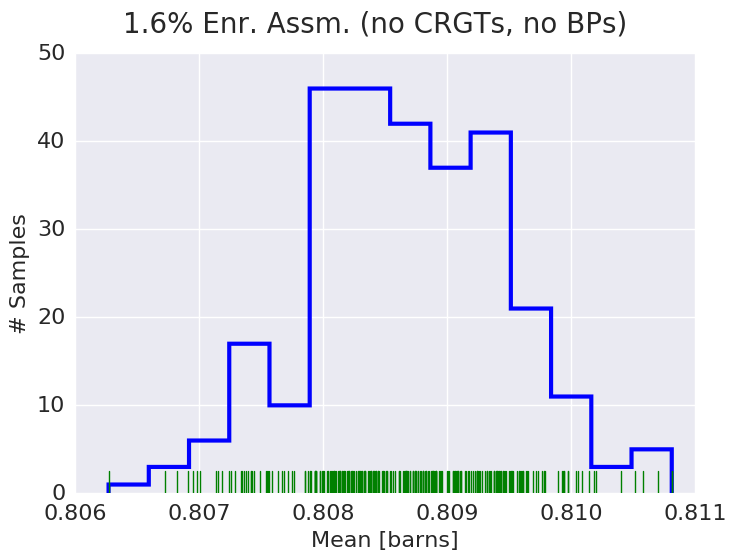
\includegraphics[width=\linewidth]{figures/patterns/assm-1.6-inf/hist-kde-rug/assm-16-inf-capt-1}
  \caption{}
  \label{fig:chap9-hist-assm-1.6-inf-capt}
\end{subfigure}%
\begin{subfigure}{0.5\textwidth}
  \centering
  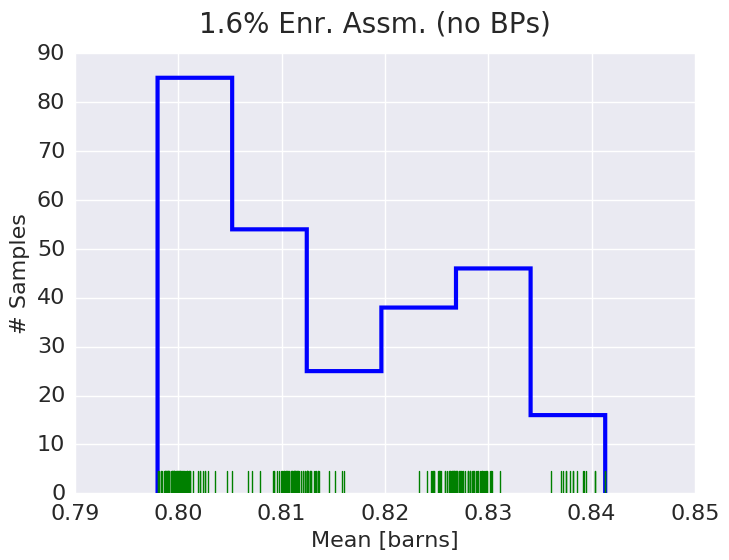
\includegraphics[width=\linewidth]{figures/patterns/assm-1.6/hist-kde-rug/assm-16-capt-1}
  \caption{}
  \label{fig:chap9-hist-assm-1.6-capt}
\end{subfigure}
\begin{subfigure}{0.5\textwidth}
  \centering
  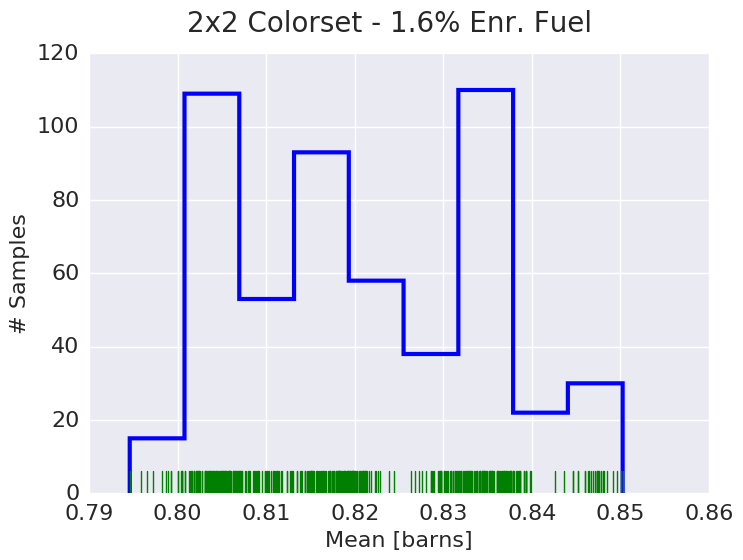
\includegraphics[width=\linewidth]{figures/patterns/2x2/hist-kde-rug/16-enr-capt-1}
  \caption{}
  \label{fig:chap9-hist-2x2-1.6-capt}
\end{subfigure}%
\begin{subfigure}{0.5\textwidth}
  \centering
  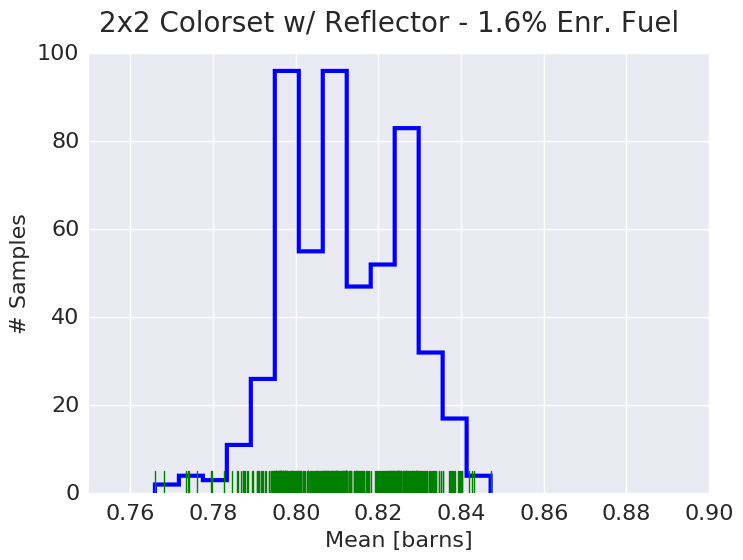
\includegraphics[width=\linewidth]{figures/patterns/reflector/hist-kde-rug/16-enr-capt-1}  \caption{}
  \label{fig:chap9-hist-reflector-1.6-capt}
\end{subfigure}
\begin{subfigure}{0.5\textwidth}
  \centering
  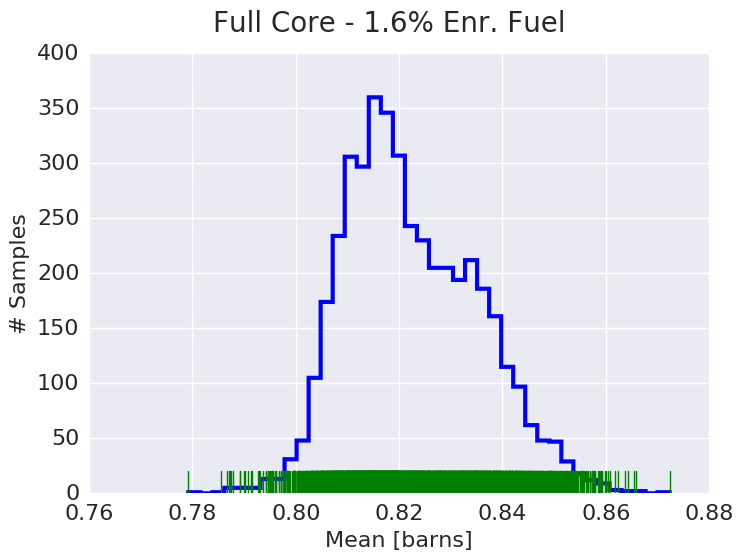
\includegraphics[width=\linewidth]{figures/patterns/full-core/hist-kde-rug/16-enr-capt-1} \caption{}
  \label{fig:chap9-hist-full-core-1.6-capt}
\end{subfigure}
\caption[Histogram of U-238 capture MGXS for 1.6\% enriched fuel]{Histograms of U-238 capture \ac{MGXS} (group 1 of 2) for 1.6\% enriched fuel.}
\label{fig:chap9-hist-1.6-capt}
\end{figure}

\begin{figure}[h!]
\centering
\begin{subfigure}{0.5\textwidth}
  \centering
  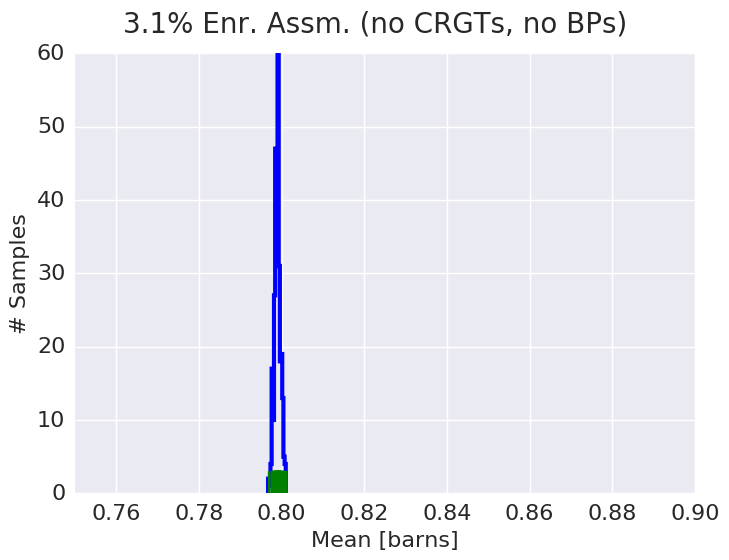
\includegraphics[width=\linewidth]{figures/patterns/assm-3.1-inf/hist-kde-rug/assm-31-inf-capt-1}
  \caption{}
  \label{fig:chap9-hist-assm-3.1-inf-capt}
\end{subfigure}%
\begin{subfigure}{0.5\textwidth}
  \centering
  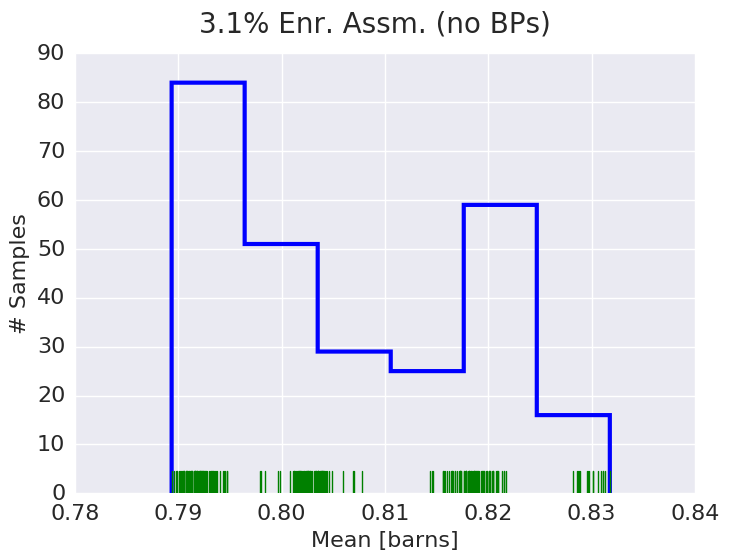
\includegraphics[width=\linewidth]{figures/patterns/assm-3.1/hist-kde-rug/assm-31-capt-1}
  \caption{}
  \label{fig:chap9-hist-assm-3.1-capt}
\end{subfigure}
\begin{subfigure}{0.5\textwidth}
  \centering
  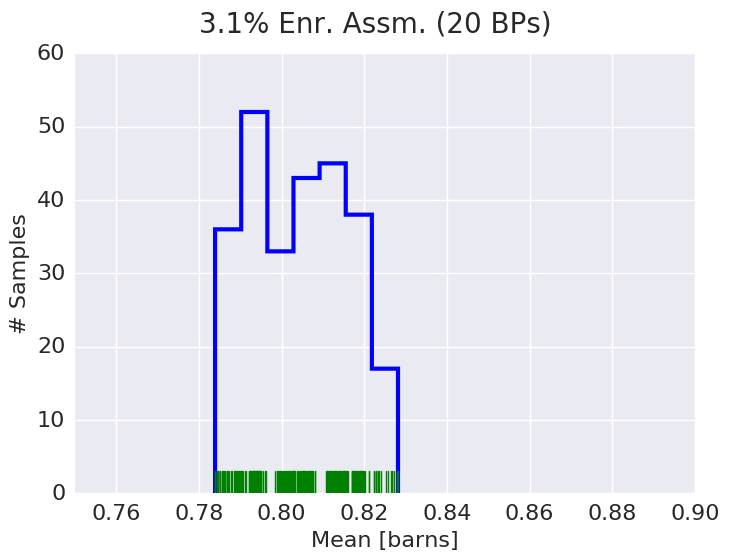
\includegraphics[width=\linewidth]{figures/patterns/assm-3.1-20BPs/hist-kde-rug/assm-31-20BPs-capt-1}
  \caption{}
  \label{fig:chap9-hist-assm-3.1-20BPs-capt}
\end{subfigure}%
\begin{subfigure}{0.5\textwidth}
  \centering
  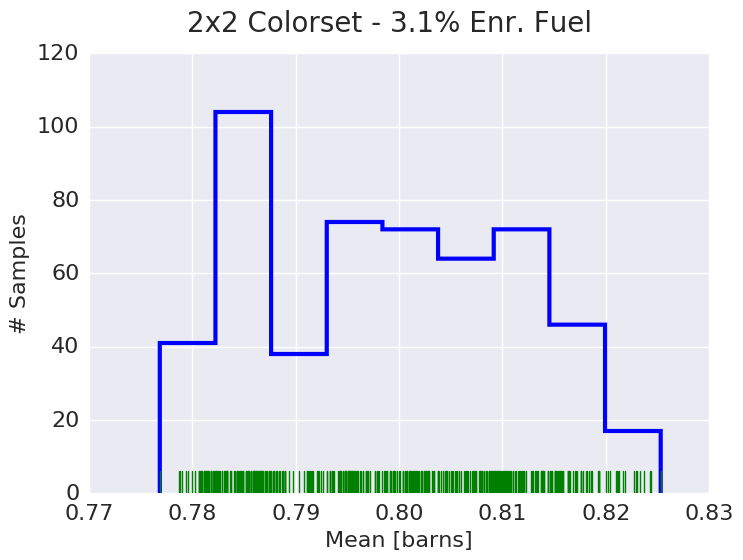
\includegraphics[width=\linewidth]{figures/patterns/2x2/hist-kde-rug/31-enr-capt-1}
  \caption{}
  \label{fig:chap9-hist-2x2-3.1-capt}
\end{subfigure}
\begin{subfigure}{0.5\textwidth}
  \centering
  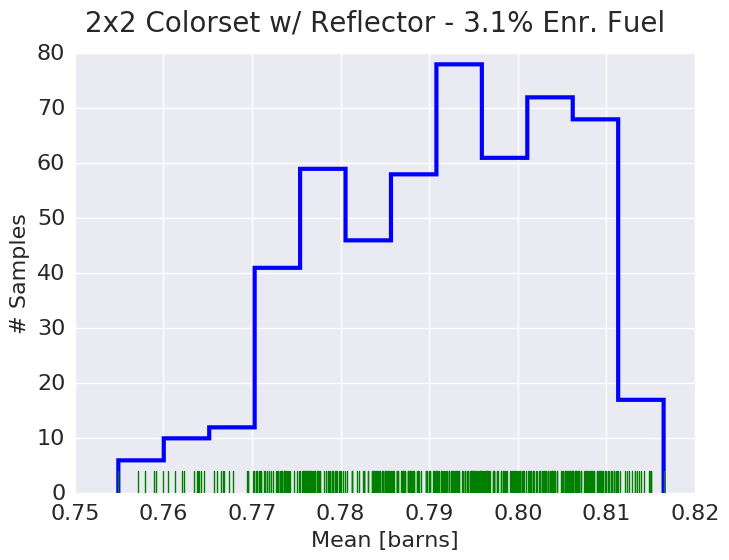
\includegraphics[width=\linewidth]{figures/patterns/reflector/hist-kde-rug/31-enr-capt-1}  \caption{}
  \label{fig:chap9-hist-reflector-3.1-capt}
\end{subfigure}%
\begin{subfigure}{0.5\textwidth}
  \centering
  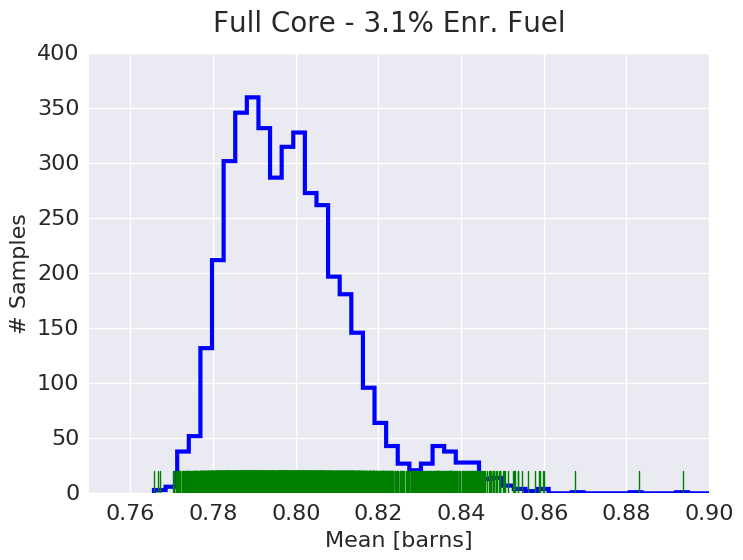
\includegraphics[width=\linewidth]{figures/patterns/full-core/hist-kde-rug/31-enr-capt-1} \caption{}
  \label{fig:chap9-hist-full-core-3.1-capt}
\end{subfigure}
\caption[Histogram of U-238 capture MGXS for 3.1\% enriched fuel]{Histograms of U-238 capture \ac{MGXS} (group 1 of 2) for 3.1\% enriched fuel.}
\label{fig:chap9-hist-3.1-capt}
\end{figure}

\noindent The further addition of \acp{BP} to the 3.1\% enriched fuel assembly ``smears'' or disperses the four clusters of U-238 capture \ac{MGXS} in Fig.~\ref{fig:chap9-hist-assm-3.1-20BPs-capt}. In addition, the \ac{MGXS} are shifted downwards by $\sim$0.005 barns (or $\sim$0.5\%) with respect to the assembly without \acp{BP}.

The inter-assembly interfaces in the 2$\times$2 colorset benchmark results in a further ``smearing'' of the clusters for both enrichments in Figs.~\ref{fig:chap9-hist-2x2-1.6-capt} and~\ref{fig:chap9-hist-2x2-3.1-capt}. It should be noted that there are twice as many samples (\textit{e.g.}, 528 fuel pin instances for each enrichment) in the colorsets than the individual fuel assemblies. Hence, it is more challenging to distinguish clusters from the rug plots for the larger colorset benchmarks. Nonetheless, the histograms indicate the continuing presence of four distinct clusters for both enrichments, though they are easier to identify for the 1.6\% enriched fuel pins (in assemblies without \acp{BP}). The \ac{MGXS} are generally shifted higher by $\sim$0.01 barns for the 1.6\% enriched pins, and down by $\sim$0.0075 barns for the 3.1\% enriched pins, with respect to the individual fuel assemblies.

The introduction of a reflector to the 2$\times$2 colorset leads to very different empirical distributions for the two fuel enrichments in Figs.~\ref{fig:chap9-hist-reflector-1.6-capt} and~\ref{fig:chap9-hist-reflector-3.1-capt}. The reason for this is that symmetry is broken with the inclusion of the reflector. In particular, both of the 3.1\% enriched assemblies are symmetrically adjacent to the reflector, and therefore have identical pin-wise \ac{MGXS}. However, one of the 1.6\% enriched assemblies is corner adjacent to the reflector while the other is located within the interior of the colorset. Nevertheless, some general observations can be made from the data. First, the \ac{MGXS} are generally even more ``smeared'' for both enrichments than is the case for the colorset without a reflector. The histogram indicates the existence of at least three clusters for the 1.6\% enriched pins, with a similar but less concentrated three-way clustering for the 3.1\% enriched pins. Finally, the lowest pin-wise \ac{MGXS} for both enrichments are $\sim$0.025 barns (or $\sim$3\%) less than those in the colorset without a reflector. This may be due to a harder spectrum in fuel pins along the left and top boundaries which have periodic \acp{BC} in the colorset without a reflector, but reflective \acp{BC} for the reflected benchmark.

%-trends w/ reflector
%  -pins with smallest \ac{MGXS} shifted down by $\sim$0.025 barns
%  -perhaps the uncertainties are just larger for the reflector and those pins are outliers??

The quarter core \ac{BEAVRS} model has the smoothest varying empirical distributions of any of the benchmarks in Figs.~\ref{fig:chap9-hist-full-core-1.6-capt} and~\ref{fig:chap9-hist-full-core-3.1-capt}. This is due in part to the fact that there are over 8$\times$ more samples for each fuel enrichment than are present for the colorsets\footnote{There are 4,332 1.6\%, 4,260 2.4\% and 4,236 3.1\% enriched fuel pins in the quarter core model.}. The most notable observation is that the distributions appear to first order to be bimodal with large peaks centered at approximately 0.815 and 0.83 barns, and 0.785 and 0.805 barns, for the 1.6\% and 3.1\% enriched pins, respectively. The distribution for the 3.1\% enriched fuel pins has an additional smaller shoulder centered at 0.83 barns. Additionally, a few 3.1\% enriched pins have significantly greater \ac{MGXS} between 0.86 and 0.9 barns. This is likely due to the fact that the 3.1\% enriched assemblies surround the exterior of the core configuration. As a result, the flux is more strongly shielded in the U-238 resonance energies for 3.1\% enriched pins adjacent to the baffle/reflector than the 1.6\% enriched pins in the interior, resulting in some larger ``outlier'' pin-wise \ac{MGXS}.

Finally, it should be noted that the microscopic U-238 capture \ac{MGXS} are generally 0.01 -- 0.02 barns (or 1.25 -- 2.5\%) larger for the 1.6\% than the 3.1\% enriched fuel pins for each respective benchmark, including the infinite lattice. These results indicate that the flux is less shielded at resonance energies for the lesser enriched fuel, perhaps due to a slightly larger fraction of neutrons up-scattering from group two to one due to the smaller probability of fission. This variation of U-238 capture \ac{MGXS} with fuel enrichment remains true even for the quarter core \ac{BEAVRS} model. However, the single largest U-238 capture \ac{MGXS} is in a 3.1\% enriched fuel pin corner adjacent to the baffle, which likely has the softest spectrum of any pin due to the nearby reflector.

%This is counter-intuitive to what one might expect -- namely, that the removal of neutrons in U-238 capture resonances would shield the flux in energy intervals where the U-238 capture cross section is greatest, reducing the flux-weighted energy-integrated \ac{MGXS}. However, 

%This may be due to a more strongly peaked ``rim effect'' of U-238 capture along the pin-moderator interface in the 1.6\% enriched pins. As a result, the flux at the interior of the lesser enriched pins may be less shielded  at resonance energies, leading to a slightly larger 

%This effect is likely due to the removal of neutrons in U-238 capture resonances as they traverse each fuel pin. As a result, the flux in those energy intervals where the U-238 capture cross section is greatest and hence reducing the flux-weighted energy-integrated \ac{MGXS}. Interestingly, this impact  

\begin{emphbox}
\textbf{The dispersion of pin-wise U-238 capture \ac{MGXS} is highly uneven and structured. Core heterogeneities such as \acp{CRGT}, \acp{BP} and reflectors induce clustering due to spatial self-shielding effects such as differential moderation, which are observed from empirical distributions of the pin-wise \ac{MGXS}.}
\end{emphbox}

%%%%%%%%%%%%%%%%%%%%%%%%%%%%%%%%%%
\subsubsection{U-235 Fission MGXS}
\label{subsubsec:chap9-histograms-fiss}

The pin-wise microscopic U-235 fission \ac{MGXS} for 1.6\% and 3.1\% enriched fuel pins are illustrated with histograms and rug plots in Fig.~\ref{fig:chap9-hist-1.6-fiss} and~\ref{fig:chap9-hist-3.1-fiss}, respectively. Each of the plots corresponds to an infinite lattice configuration or one of the six heterogeneous benchmarks. The trends observed in the plots can be attributed to the presence of \acp{CRGT}, \acp{BP}, assembly-assembly and/or assembly-reflector interfaces or fuel enrichment. 

\begin{figure}[h!]
\centering
\begin{subfigure}{0.5\textwidth}
  \centering
  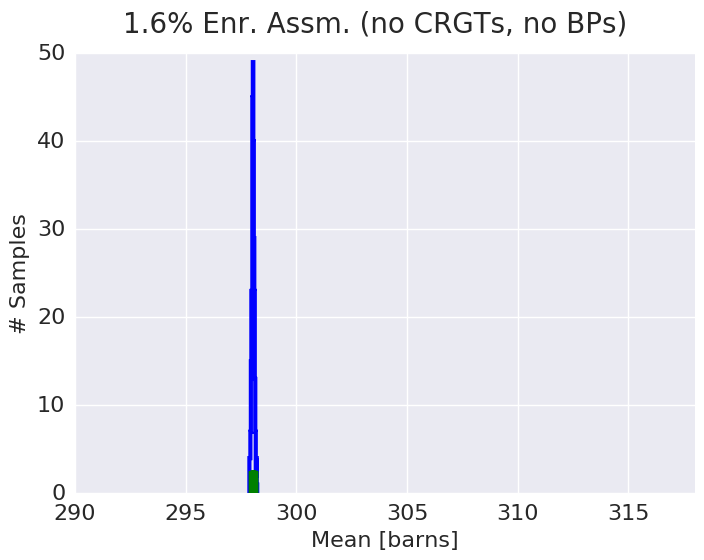
\includegraphics[width=\linewidth]{figures/patterns/assm-1.6-inf/hist-kde-rug/assm-16-inf-fiss-2}
  \caption{}
  \label{fig:chap9-hist-assm-1.6-inf-fiss}
\end{subfigure}%
\begin{subfigure}{0.5\textwidth}
  \centering
  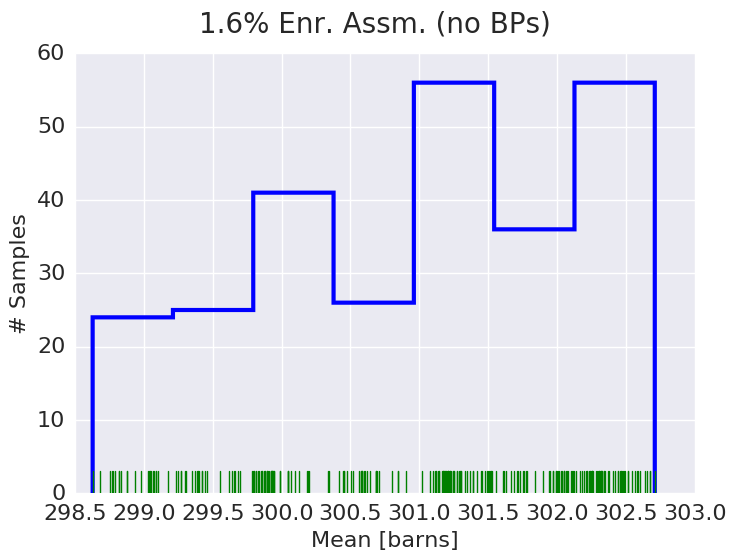
\includegraphics[width=\linewidth]{figures/patterns/assm-1.6/hist-kde-rug/assm-16-fiss-2}
  \caption{}
  \label{fig:chap9-hist-assm-1.6-fiss}
\end{subfigure}
\begin{subfigure}{0.5\textwidth}
  \centering
  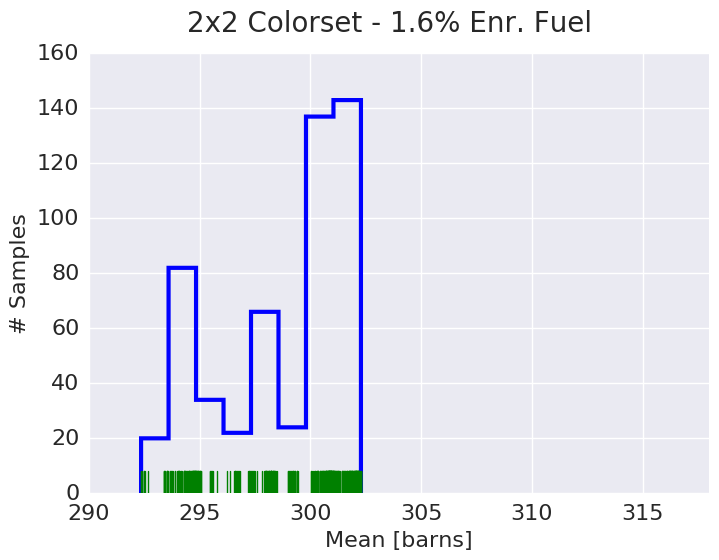
\includegraphics[width=\linewidth]{figures/patterns/2x2/hist-kde-rug/16-enr-fiss-2}
  \caption{}
  \label{fig:chap9-hist-2x2-1.6-fiss}
\end{subfigure}%
\begin{subfigure}{0.5\textwidth}
  \centering
  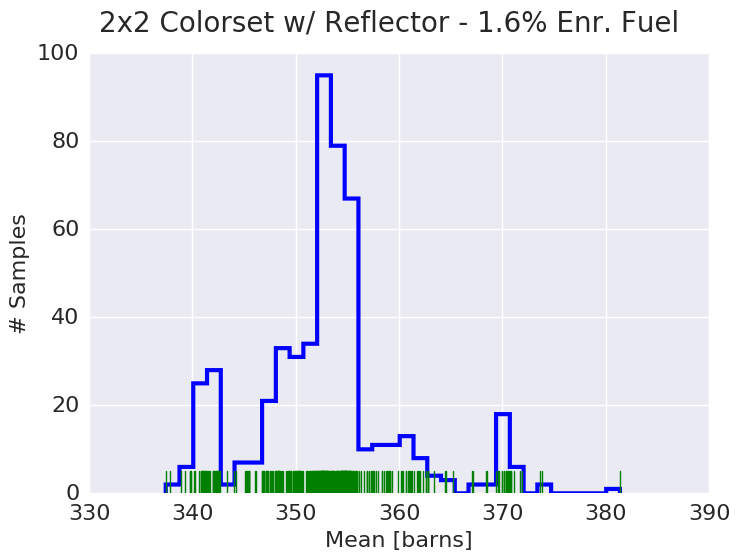
\includegraphics[width=\linewidth]{figures/patterns/reflector/hist-kde-rug/16-enr-fiss-2}  \caption{}
  \label{fig:chap9-hist-reflector-1.6-fiss}
\end{subfigure}
\begin{subfigure}{0.5\textwidth}
  \centering
  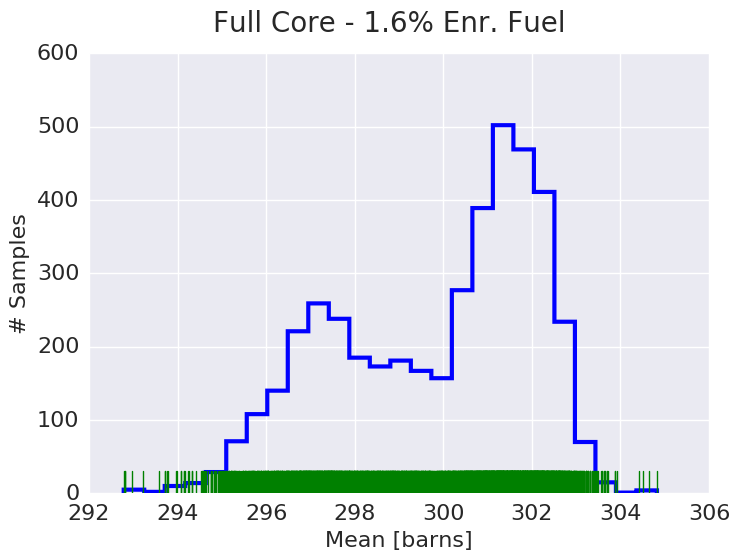
\includegraphics[width=\linewidth]{figures/patterns/full-core/hist-kde-rug/16-enr-fiss-2} \caption{}
  \label{fig:chap9-hist-full-core-1.6-fiss}
\end{subfigure}
\caption[Histogram of U-235 fission MGXS for 1.6\% enriched fuel]{Histograms of U-235 fission \ac{MGXS} (group 2 of 2) for 1.6\% enriched fuel.}
\label{fig:chap9-hist-1.6-fiss}
\end{figure}

\begin{figure}[h!]
\centering
\begin{subfigure}{0.5\textwidth}
  \centering
  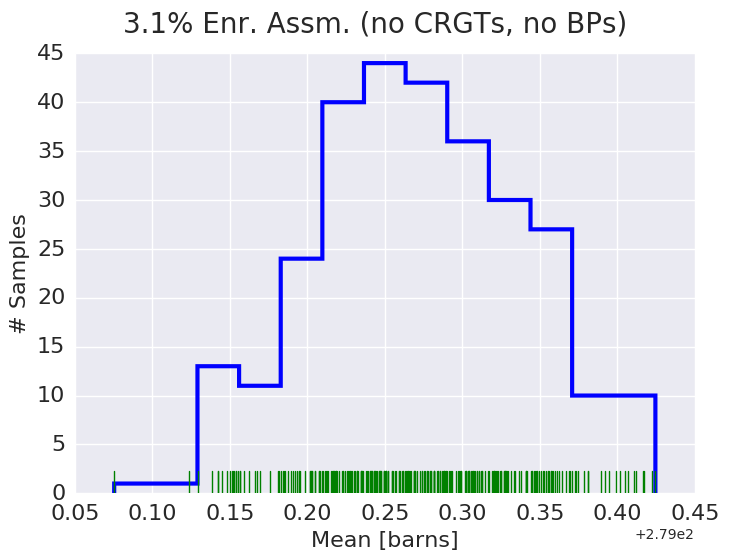
\includegraphics[width=\linewidth]{figures/patterns/assm-3.1-inf/hist-kde-rug/assm-31-inf-fiss-2}
  \caption{}
  \label{fig:chap9-hist-assm-3.1-inf-fiss}
\end{subfigure}%
\begin{subfigure}{0.5\textwidth}
  \centering
  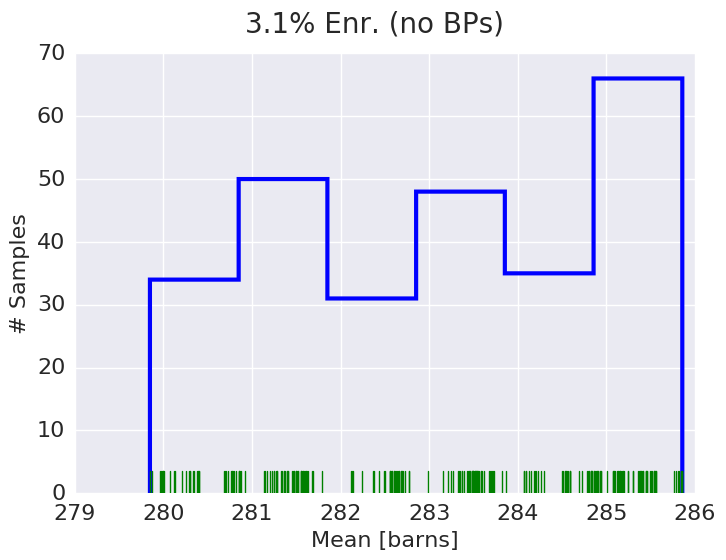
\includegraphics[width=\linewidth]{figures/patterns/assm-3.1/hist-kde-rug/assm-31-fiss-2}
  \caption{}
  \label{fig:chap9-hist-assm-3.1-fiss}
\end{subfigure}
\begin{subfigure}{0.5\textwidth}
  \centering
  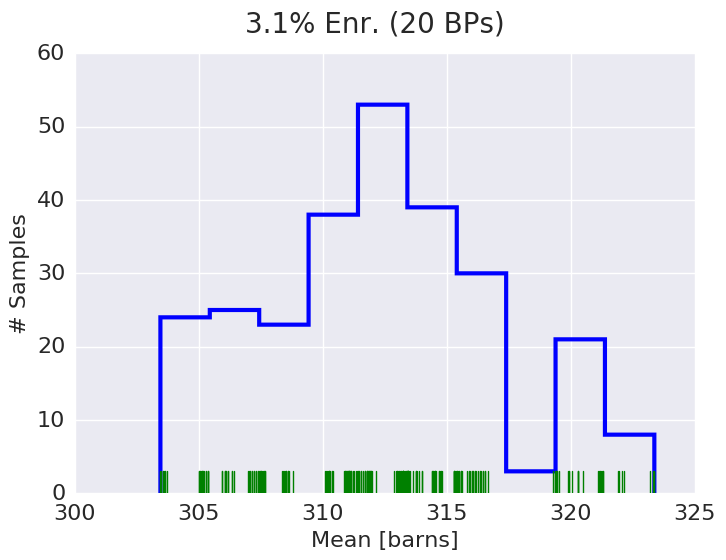
\includegraphics[width=\linewidth]{figures/patterns/assm-3.1-20BPs/hist-kde-rug/assm-31-20BPs-fiss-2}
  \caption{}
  \label{fig:chap9-hist-assm-3.1-20BPs-fiss}
\end{subfigure}%
\begin{subfigure}{0.5\textwidth}
  \centering
  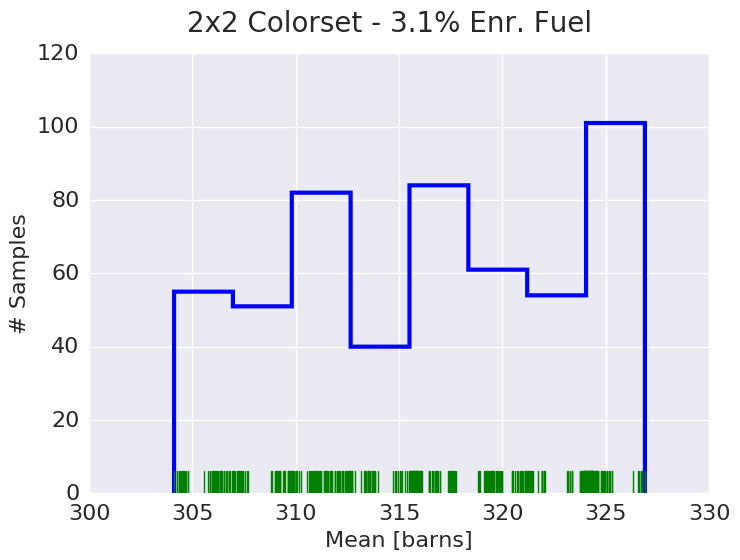
\includegraphics[width=\linewidth]{figures/patterns/2x2/hist-kde-rug/31-enr-fiss-2}
  \caption{}
  \label{fig:chap9-hist-2x2-3.1-fiss}
\end{subfigure}
\begin{subfigure}{0.5\textwidth}
  \centering
  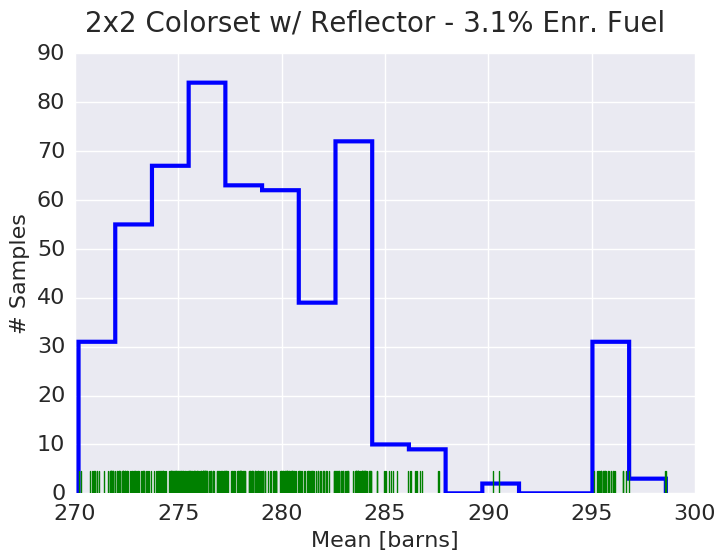
\includegraphics[width=\linewidth]{figures/patterns/reflector/hist-kde-rug/31-enr-fiss-2}  \caption{}
  \label{fig:chap9-hist-reflector-3.1-fiss}
\end{subfigure}%
\begin{subfigure}{0.5\textwidth}
  \centering
  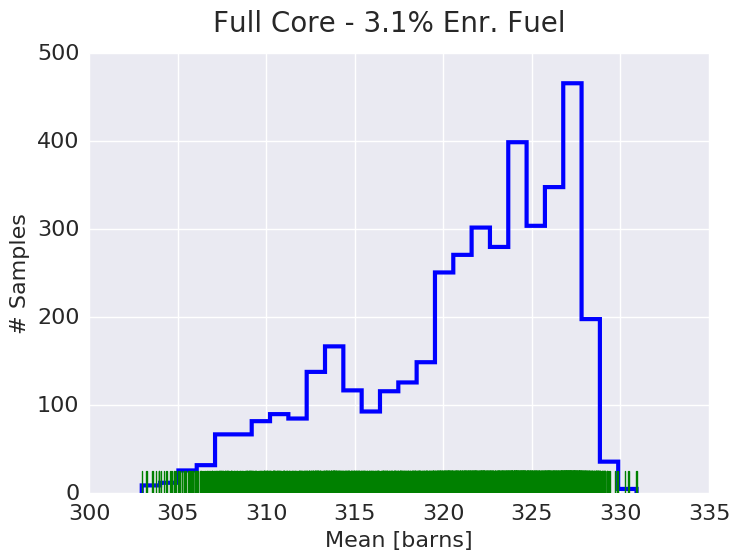
\includegraphics[width=\linewidth]{figures/patterns/full-core/hist-kde-rug/31-enr-fiss-2} \caption{}
  \label{fig:chap9-hist-full-core-3.1-fiss}
\end{subfigure}
\caption[Histogram of U-235 fission MGXS 3.1\% enriched fuel]{Histograms of U-235 fission \ac{MGXS} (group 2 of 2) for 3.1\% enriched fuel.}
\label{fig:chap9-hist-3.1-fiss}
\end{figure}

First, the U-235 fission \ac{MGXS} are over 300$\times$ larger than the U-238 capture \ac{MGXS} illustrated in the preceding section. However, the it should be recalled that the U-238 nuclide density is over 30 -- 60$\times$ larger than U-235 in the 1.6\% and 3.1\% enriched fuel, respectively. As a consequence, the clustering of either microscopic U-238 capture or the U-235 fission \ac{MGXS} is important since it will have a similarly sized impact on the corresponding macroscopic \ac{MGXS} and reaction rates.

As was observed for U-238 capture, the empirical distributions of pin-wise \ac{MGXS} for the infinite lattices in Figs.~\ref{fig:chap9-hist-assm-1.6-inf-fiss} and~\ref{fig:chap9-hist-assm-3.1-inf-fiss} are narrow and symmetric unlike the distributions for each of the heterogeneous benchmarks. Unlike the situation for U-238 capture, the introduction of \acp{CRGT} induces a more intricate clustering of the U-235 fission \ac{MGXS} in Figs.~\ref{fig:chap9-hist-assm-1.6-fiss} and~\ref{fig:chap9-hist-assm-3.1-fiss}. First, the total range of U-235 fission \ac{MGXS} in the fuel assemblies with \acp{CRGT} varies by only 1 -- 2\% as compared to more than 5\% for U-238 capture. The histograms indicate the presence of roughly three clusters of \ac{MGXS} which are separated by 1 -- 2 barns for both fuel enrichments. The rug plots illustrate a more complicated dispersion, however, with a significantly more distinct concentration into approximately eight clusters for the 3.1\% enriched fuel pins. These observations indicate that U-235 fission may be more sensitive than U-238 capture to spatial self-shielding effects from the differential moderation of \acp{CRGT}, even though the impact on the resultant \ac{MGXS} is of a smaller relative magnitude. 

The further addition of \acp{BP} to the 3.1\% enriched fuel assembly results in a more distinct set of isolated clusters of U-235 fission \ac{MGXS} in Fig.~\ref{fig:chap9-hist-assm-3.1-20BPs-fiss}. In particular, there appear to be three overall clusters centered at approximately 272, 276 and 300 barns each with a number of sub-clusters. This stands in contrast to the case for U-238 capture where the presence of \acp{BP} resulted in a ``smearing'' of the clusters. In addition, the \ac{MGXS} are generally shifted downwards by 5 -- 10  barns (or 1.5 -- 3\%) with respect to the assembly without \acp{BP}. Similarly, the inter-assembly interfaces in the 2$\times$2 colorset benchmark have a similarly concentrating effect for both enrichments in Figs.~\ref{fig:chap9-hist-2x2-1.6-fiss} and~\ref{fig:chap9-hist-2x2-3.1-fiss}. The histograms reveal three clusters centered at approximately 294, 298 and 301 barns for the 1.6\% enriched pins, and four clusters centered at 271, 275, 278 and 283 barns for the 3.1\% enriched pins. Furthermore, the rug plots indicate the presence of more clusters which are more easily distinguishable than they are for the individual fuel assemblies, or for the U-238 capture \ac{MGXS} in the 2$\times$2 colorset benchmark. Finally, the \ac{MGXS} in the colorset are generally shifted downwards by 3 -- 6  barns (or 1 -- 2\%) with respect to the individual fuel assemblies.

The introduction of a reflector to the 2$\times$2 colorset leads to very different empirical distributions for the two fuel enrichments in Figs.~\ref{fig:chap9-hist-reflector-1.6-fiss} and~\ref{fig:chap9-hist-reflector-3.1-fiss}. As was noted in Sec.~\ref{subsubsec:chap9-histograms-capt}, the reason for this is that symmetry is broken with the inclusion of the reflector. A first observation is that the empirical distributions of U-235 fission \ac{MGXS} for the two enrichments differ much more profoundly than they do for U-238 capture. The histogram for the 1.6\% enriched pins indicate perhaps six primary clusters centered at 294, 298, 301, 304, 306 and 310 barns, though the rug plot certainly indicates the presence of even further sub-clusters. The histogram for the 3.1\% enriched pins indicate perhaps four clusters roughly centered at 276, 284, 290 and 296 barns, though the intervals between these apparent clusters contain many additional samples, complicating the analysis. Finally, the largest U-235 fission \ac{MGXS} are approximately 315 and 300 barns for the 1.6\% and 3.1\% enriched pins in the colorset, respectively, about 15 barns (or 5\%) greater than the largest \ac{MGXS} for the colorset without a reflector. This is due to the softer flux spectrum experienced by those pins adjacent to the reflector.

As was noted for the U-238 capture \ac{MGXS}, the quarter core \ac{BEAVRS} model has the smoothest varying empirical distributions of any of the benchmarks in Figs.~\ref{fig:chap9-hist-full-core-1.6-fiss} and~\ref{fig:chap9-hist-full-core-3.1-fiss}. The most notable observation is that the distributions appear to first order to be bimodal and trimodal with large peaks centered at approximately 297 and 302 barns, and 278, 283 and 284 barns, for the 1.6\% and 3.1\% enriched pins, respectively. The two peaks are more clearly discernible for the 1.6\% enriched fuel pins. This effect may be due to an increase in moderation for those 1.6\% enriched assemblies that are only one assembly removed from the reflector as compared to those in the interior of the core. Furthermore, the range of \ac{MGXS} in the quarter core model only spans 10 -- 15 barns (or 5\%) as compared to the 20 -- 25 barns for the 2$\times$ colorset benchmark. This is likely due to the presence of a stainless steel baffle separating the assemblies on the exterior of the \ac{BEAVRS} model from the water reflector. The baffle dampens the additional moderation experienced by those pins nearest the reflector in the \ac{BEAVRS} model with respect to those in the 2$\times$2 colorset with a reflector but no baffle.

Finally, it should be noted that the microscopic U-235 fission \ac{MGXS} are generally 18 -- 22 barns (or 6+\%) larger for the 1.6\% than the 3.1\% enriched fuel pins for each respective benchmark, including the infinite lattice. These results indicate that the flux is more strongly moderated for the lesser enriched fuel, perhaps due to the smaller probability of fission. This variation of U-235 fission \ac{MGXS} with fuel enrichment remains true even for the quarter core \ac{BEAVRS} model. 

\begin{emphbox}
\textbf{The presence of core heteorgeneities induce more clearly defined clustering of pin-wise U-235 fission \ac{MGXS} than is observed for U-238 capture (in 2-group data). However, the population of pin-wise U-235 fission \ac{MGXS} only disperse by 1 -- 2\%, while the U-238 capture \ac{MGXS} dispersion is $\sim$5\%.}
\end{emphbox}

%%%%%%%%%%%%%%%%%%%%%%%%%%%%%%%%%%%%%%%%%%%%%%%%%%%%%
\subsection{Quantile-Quantile Plots of Pin-Wise MGXS}
\label{subsec:chap9-qq-plots}

This section illustrates the deviation from normality of pin-wise \ac{MGXS} with \ac{Q-Q} plots. A \ac{Q-Q} plot is used to compare two datasets drawn from different probability distributions. In particular, the quantiles from one dataset are plotted against the quantiles of a second dataset in an $(x,y)$ scatter plot\footnote{A \textit{quantile} is the point at which some fraction of the data falls below a given value. For example, the 10\% quantile is the point at which 10\% of the data is below the point and 90\% is above it.}. If the two distributions are similar, the data points will lie along the $y = x$ reference line. Departures from $y = x$ indicate dis-similarities between the distributions, such as shifts in location or scale, changes in symmetry, and outliers. 

\interfootnotelinepenalty=10000

In this section, the theoretical quantiles for a normal distribution are plotted against empirical quantiles found from the empirical distribution of pin-wise U-238 capture and U-235 fission \ac{MGXS}. These \ac{Q-Q} plots illustrate the deviation from normality for the data as heterogeneities are introduced to the benchmark models. It should be noted that standardization is first applied to the \ac{MGXS} data so that it can be compared to theoretical quantiles from a standard normal distribution $\mathcal{N}(0,1)$ in the \ac{Q-Q} plots. The visualizations are presented for an infinite lattice as well as the six heterogeneous benchmarks for both 1.6\% and 3.1\% enriched fuel. The random samples in each visualization (\textit{e.g.}, each blue data point) correspond to a single fuel pin instance in the corresponding benchmark model. In addition, each plot highlights the $p$-value\footnote{The $p$-value is used in null hypothesis significance testing and measures the likelihood of an observation as or more extreme than the given one. In this section, the null hypothesis is that pin-wise \ac{MGXS} data is drawn from a normal distribution. To test this hypothesis, a significance level $\alpha$ is chosen (\textit{e.g.} 1\%) and compared with the $p$-value of the Shapiro-Wilk normality test. If $p < \alpha$ then the null hypothesis is rejected (\textit{i.e.}, the dataset was not drawn from a normal distribution); otherwise, it cannot be rejected.} for the Shapiro-Wilk test of normality~\cite{shapiro1965analysis} computed using the Python \texttt{scipy.stats} package~\cite{jones2011scipy}.

%%%%%%%%%%%%%%%%%%%%%%%%%%%%%%%%%%
\subsubsection{U-238 Capture MGXS}
\label{subsubsec:chap9-qq-plots-capt}

The pin-wise microscopic U-238 capture \ac{MGXS} for 1.6\% and 3.1\% enriched fuel pins are illustrated with histograms and rug plots in Fig.~\ref{fig:chap9-qq-1.6-capt} and~\ref{fig:chap9-qq-3.1-capt}, respectively. Each of the plots corresponds to an infinite lattice configuration or one of the six heterogeneous benchmarks. The trends observed in the plots can be attributed to the presence of \acp{CRGT}, \acp{BP}, assembly-assembly and/or assembly-reflector interfaces or fuel enrichment. 

\begin{figure}[h!]
\centering
\begin{subfigure}{0.5\textwidth}
  \centering
  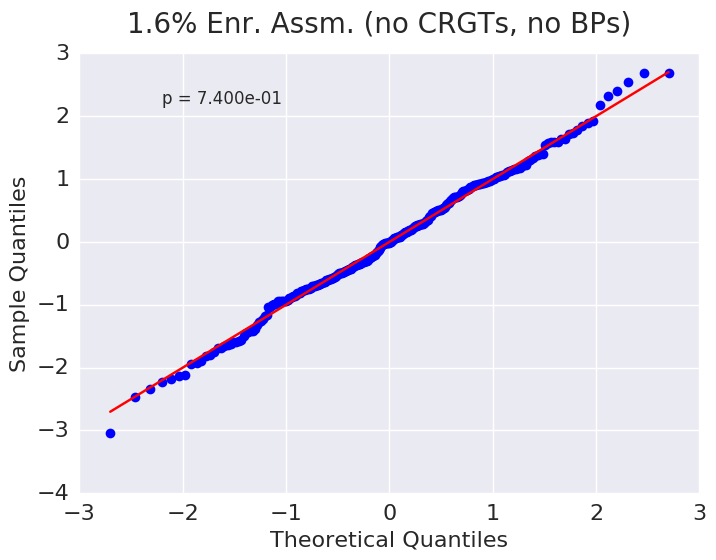
\includegraphics[width=\linewidth]{figures/patterns/assm-1.6-inf/quantile/assm-16-inf-capt-1}
  \caption{}
  \label{fig:chap9-qq-assm-1.6-inf-capt}
\end{subfigure}%
\begin{subfigure}{0.5\textwidth}
  \centering
  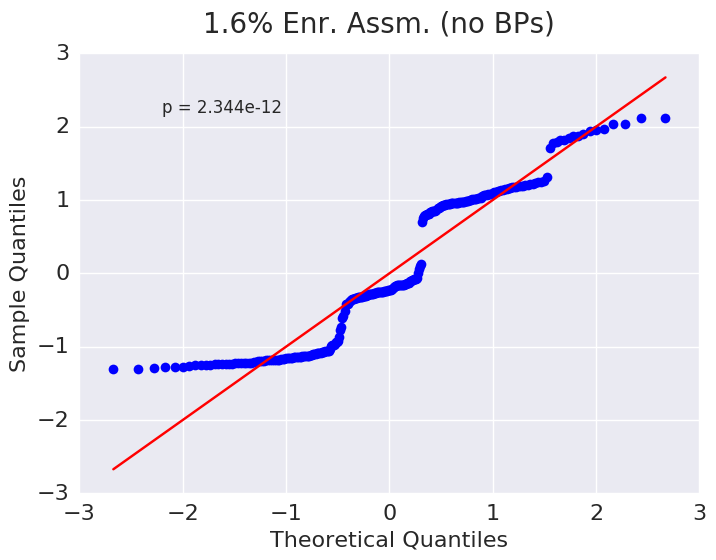
\includegraphics[width=\linewidth]{figures/patterns/assm-1.6/quantile/assm-16-capt-1}
  \caption{}
  \label{fig:chap9-qq-assm-1.6-capt}
\end{subfigure}
\begin{subfigure}{0.5\textwidth}
  \centering
  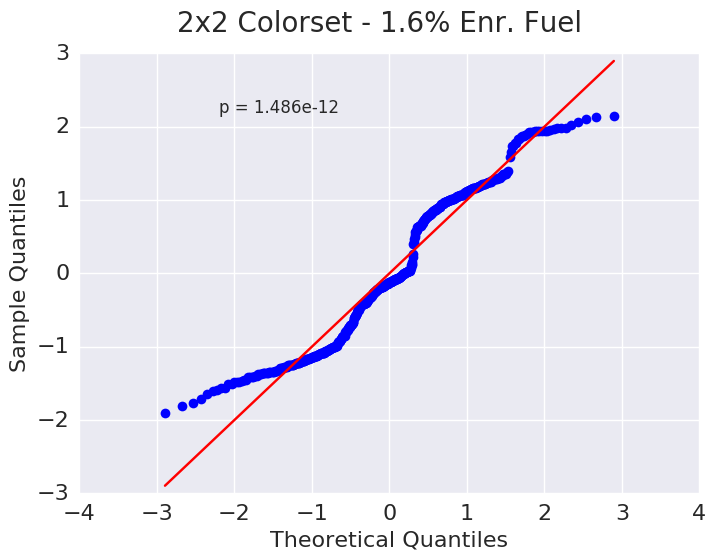
\includegraphics[width=\linewidth]{figures/patterns/2x2/quantile/16-enr-capt-1}
  \caption{}
  \label{fig:chap9-qq-2x2-1.6-capt}
\end{subfigure}%
\begin{subfigure}{0.5\textwidth}
  \centering
  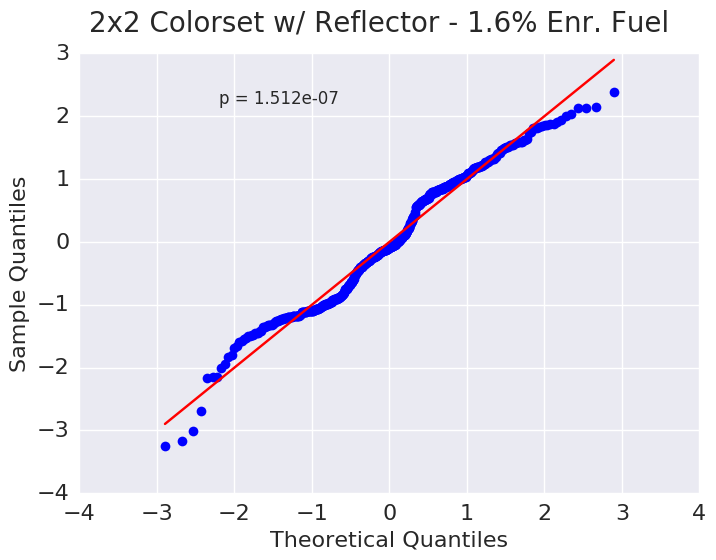
\includegraphics[width=\linewidth]{figures/patterns/reflector/quantile/16-enr-capt-1}  \caption{}
  \label{fig:chap9-qq-reflector-1.6-capt}
\end{subfigure}
\begin{subfigure}{0.5\textwidth}
  \centering
  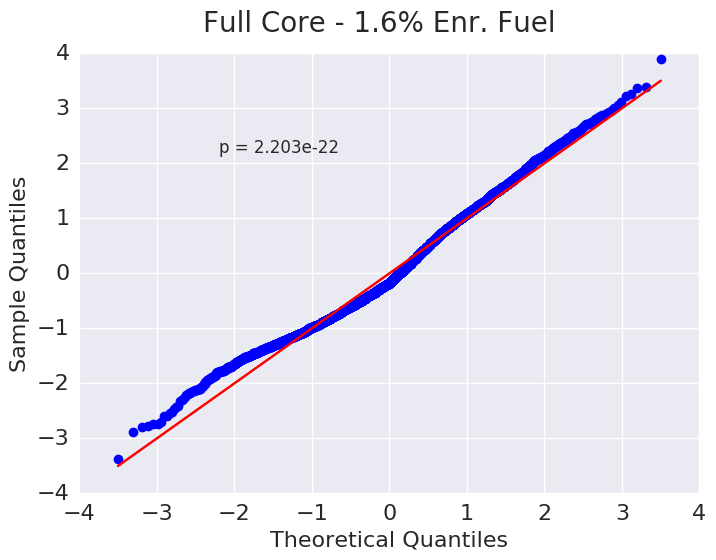
\includegraphics[width=\linewidth]{figures/patterns/full-core/quantile/16-enr-capt-1} \caption{}
  \label{fig:chap9-qq-full-core-1.6-capt}
\end{subfigure}
\caption[Q-Q plots of U-238 capture MGXS for 1.6\% enriched fuel]{\ac{Q-Q} plots of U-238 capture \ac{MGXS} (group 1 of 2) for 1.6\% enriched fuel.}
\label{fig:chap9-qq-1.6-capt}
\end{figure}

\begin{figure}[h!]
\centering
\begin{subfigure}{0.5\textwidth}
  \centering
  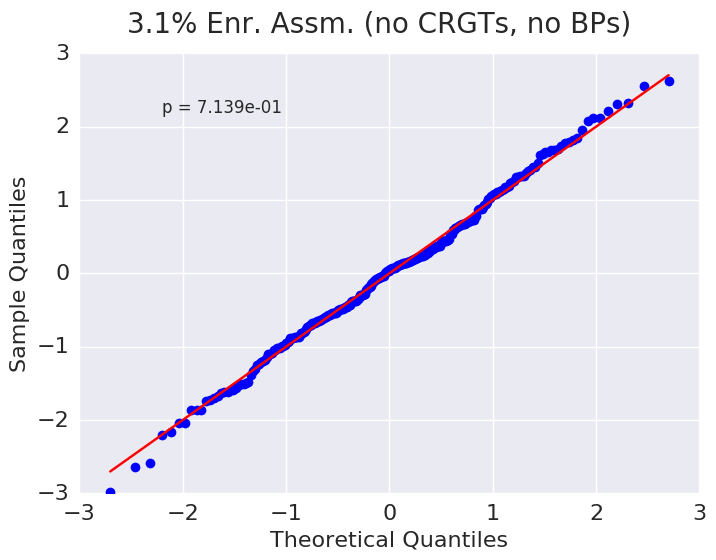
\includegraphics[width=\linewidth]{figures/patterns/assm-3.1-inf/quantile/assm-31-inf-capt-1}
  \caption{}
  \label{fig:chap9-qq-assm-3.1-inf-capt}
\end{subfigure}%
\begin{subfigure}{0.5\textwidth}
  \centering
  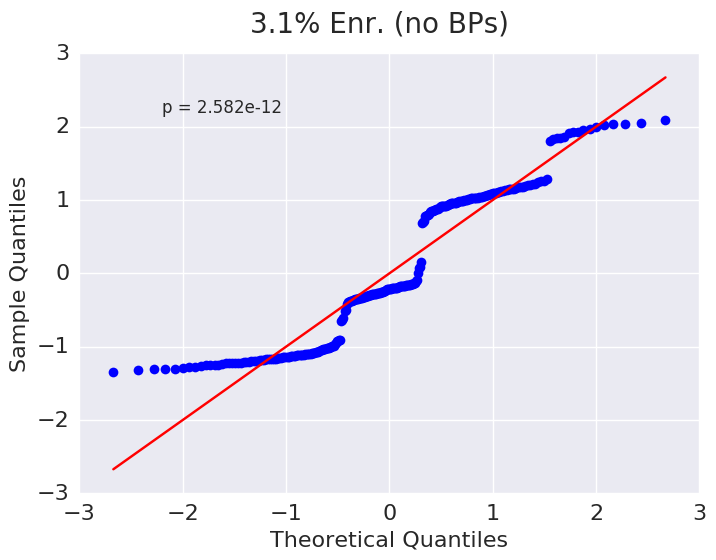
\includegraphics[width=\linewidth]{figures/patterns/assm-3.1/quantile/assm-31-capt-1}
  \caption{}
  \label{fig:chap9-qq-assm-3.1-capt}
\end{subfigure}
\begin{subfigure}{0.5\textwidth}
  \centering
  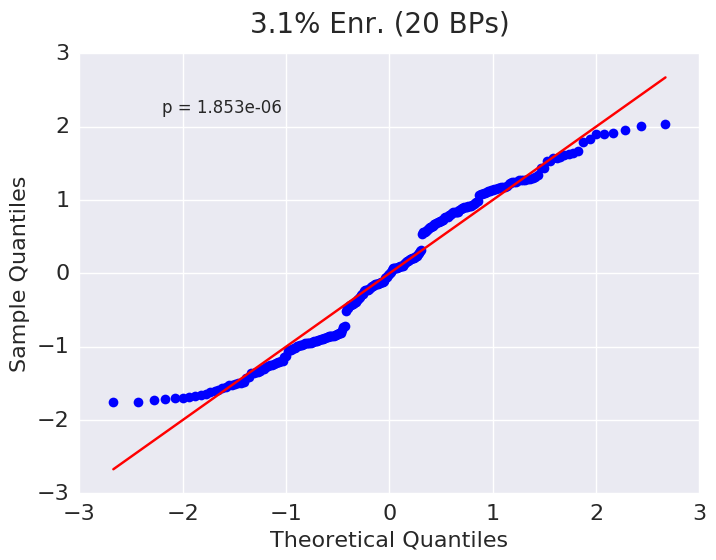
\includegraphics[width=\linewidth]{figures/patterns/assm-3.1-20BPs/quantile/assm-31-20BPs-capt-1}
  \caption{}
  \label{fig:chap9-qq-assm-3.1-20BPs-capt}
\end{subfigure}%
\begin{subfigure}{0.5\textwidth}
  \centering
  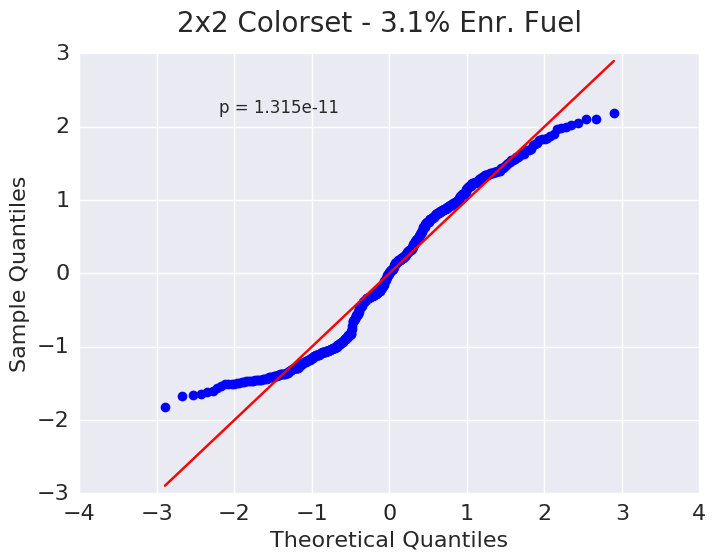
\includegraphics[width=\linewidth]{figures/patterns/2x2/quantile/31-enr-capt-1}
  \caption{}
  \label{fig:chap9-qq-2x2-3.1-capt}
\end{subfigure}
\begin{subfigure}{0.5\textwidth}
  \centering
  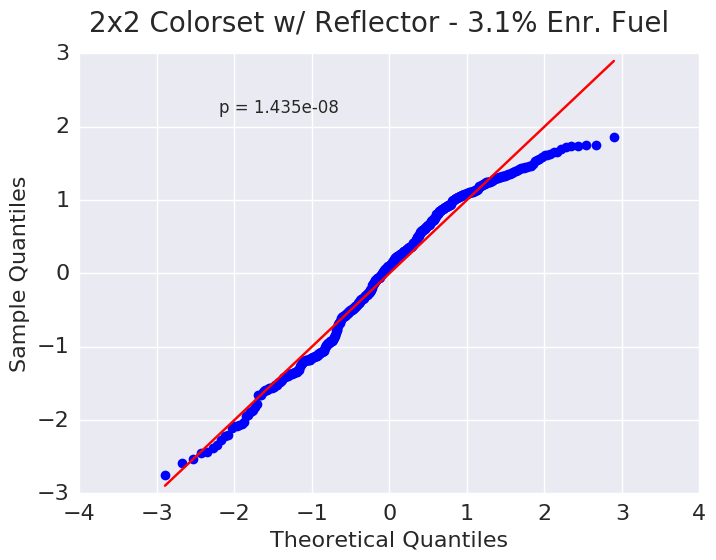
\includegraphics[width=\linewidth]{figures/patterns/reflector/quantile/31-enr-capt-1}  \caption{}
  \label{fig:chap9-qq-reflector-3.1-capt}
\end{subfigure}%
\begin{subfigure}{0.5\textwidth}
  \centering
  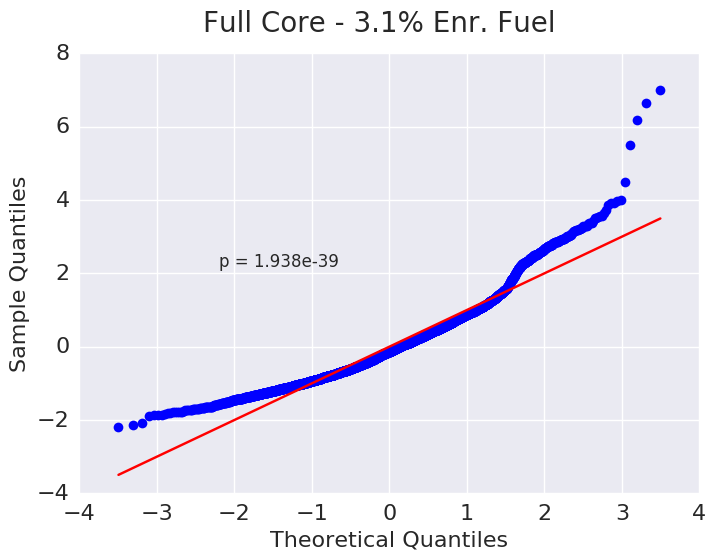
\includegraphics[width=\linewidth]{figures/patterns/full-core/quantile/31-enr-capt-1} \caption{}
  \label{fig:chap9-qq-full-core-3.1-capt}
\end{subfigure}
\caption[Q-Q plots of U-238 capture MGXS for 3.1\% enriched fuel]{\ac{Q-Q} plots of U-238 capture \ac{MGXS} (group 1 of 2) for 3.1\% enriched fuel.}
\label{fig:chap9-qq-3.1-capt}
\end{figure}

As was hypothesized earlier, the datasets for the infinite lattices in Figs.~\ref{fig:chap9-qq-assm-1.6-inf-capt} and~\ref{fig:chap9-qq-assm-3.1-inf-capt} appear to be from a normal distribution since they lie very close to the $y = x$ reference line. In addition, the $p$-values are greater than 0.7, well above commonly used significance levels; thus one would not reject the null hypothesis that the data is from a normal distribution. The addition of \acp{CRGT} leads to a clear deviation from normality in Figs.~\ref{fig:chap9-qq-assm-1.6-capt} and~\ref{fig:chap9-qq-assm-3.1-capt}, with four ``shoulders'' representing the four clusters highlighted in Sec.~\ref{subsec:chap9-histograms} for these single assembly benchmarks. The presence of \acp{BP} seems to result in more shoulders in Fig.~\ref{fig:chap9-qq-assm-3.1-20BPs-capt} corresponding to the various clusters identified in Fig.~\ref{fig:chap9-hist-assm-3.1-20BPs-capt}. 

At first glance, the larger number of data points (\textit{e.g.}, fuel pin instances) in the \ac{Q-Q} plots for the larger colorset and quarter core benchmarks appears to hide any underlying structure. Although the data points may appear to lie closer to the $y = x$ line for the larger benchmarks, this does not necessarily indicate that the data is more likely to have been drawn from a normal distribution. Indeed, smoothly varying deviations from $y = x$ exhibited in the larger datasets results in smaller $p$-values for the colorset and quarter core models. Of particular note, $p$-values on the order of 10$^{-22}$ and 10$^{-39}$ arise from the data for the 1.6\% and 3.1\% enriched fuel pins, respectively, for the \ac{BEAVRS} quarter core model. These results suggest that it is highly unlikely that the data arose from a normally distributed stochastic process.

%-mention that tails above and below on lower/upper range indicate that tails of distribution are not as wide as would be expected for normal samples -- e.g., a ``tighter'' or ``narrower'' distribution
%-3.1\% enr pins in full core are tighter on bottom edge, but wider on upper edge
%  -indicative of those few ``outlier'' pins with \ac{MGXS} near 0.9 barns in Fig.~\ref{fig:chap9-hist-3.1-capt}

\begin{emphbox}
\textbf{The clustering of U-238 capture \ac{MGXS} manifests itself as ``shoulders'' in \ac{Q-Q} plots. The Shapiro-Wilks test rejects the null hypothesis that the \ac{MGXS} data is drawn from a normal distribution for all six heterogeneous benchmarks.}
\end{emphbox}

%%%%%%%%%%%%%%%%%%%%%%%%%%%%%%%%%%
\subsubsection{U-235 Fission MGXS}
\label{subsubsec:chap9-qq-plots-fiss}

The pin-wise microscopic U-235 fission \ac{MGXS} for 1.6\% and 3.1\% enriched fuel pins are illustrated with histograms and rug plots in Fig.~\ref{fig:chap9-qq-1.6-fiss} and~\ref{fig:chap9-qq-3.1-fiss}, respectively. Each of the plots corresponds to an infinite lattice configuration or one of the six heterogeneous benchmarks. The trends observed in the plots can be attributed to the presence of \acp{CRGT}, \acp{BP}, assembly-assembly and/or assembly-reflector interfaces or fuel enrichment. 

\begin{figure}[h!]
\centering
\begin{subfigure}{0.5\textwidth}
  \centering
  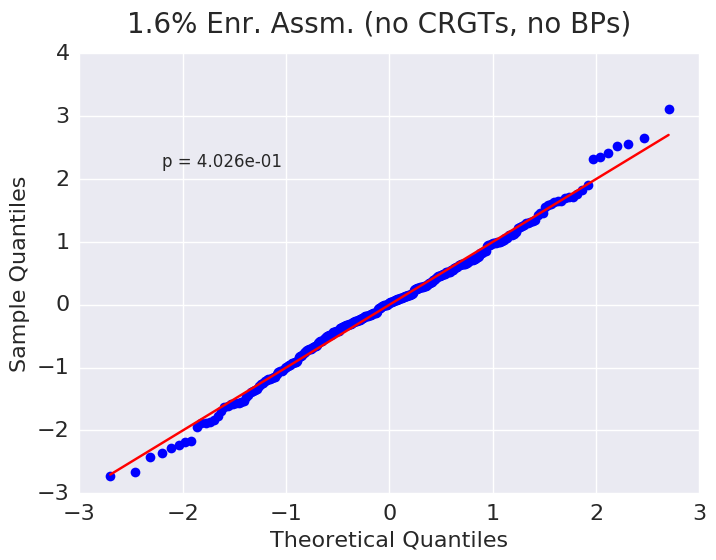
\includegraphics[width=\linewidth]{figures/patterns/assm-1.6-inf/quantile/assm-16-inf-fiss-2}
  \caption{}
  \label{fig:chap9-qq-assm-1.6-inf-fiss}
\end{subfigure}%
\begin{subfigure}{0.5\textwidth}
  \centering
  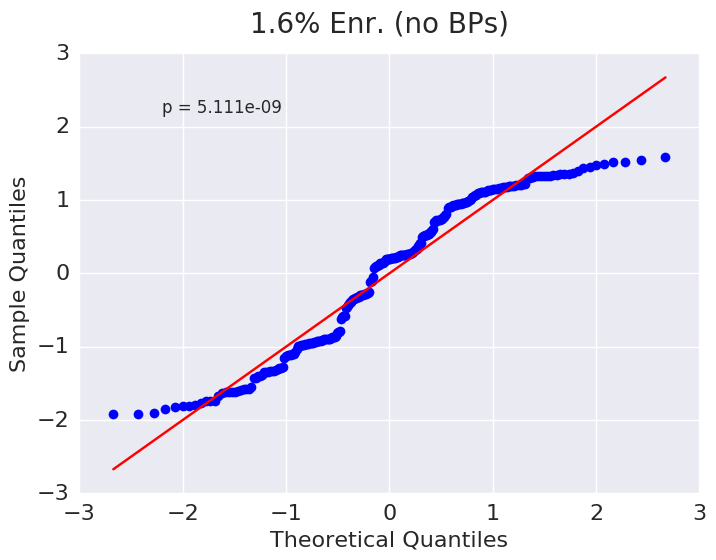
\includegraphics[width=\linewidth]{figures/patterns/assm-1.6/quantile/assm-16-fiss-2}
  \caption{}
  \label{fig:chap9-qq-assm-1.6-fiss}
\end{subfigure}
\begin{subfigure}{0.5\textwidth}
  \centering
  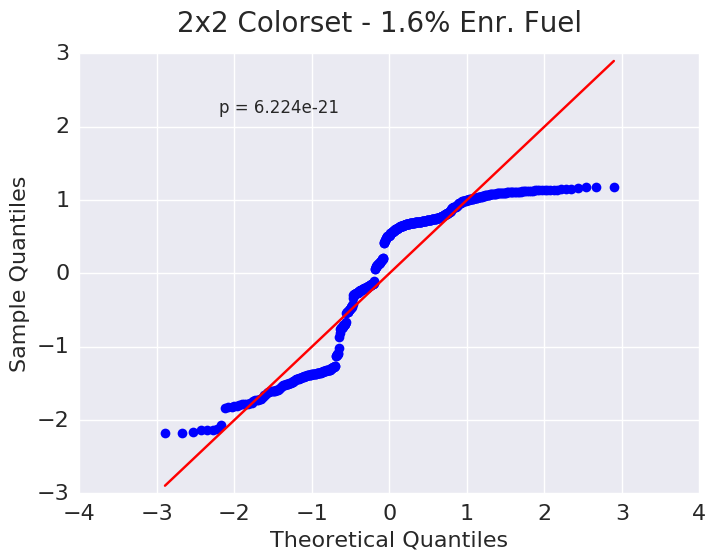
\includegraphics[width=\linewidth]{figures/patterns/2x2/quantile/16-enr-fiss-2}
  \caption{}
  \label{fig:chap9-qq-2x2-1.6-fiss}
\end{subfigure}%
\begin{subfigure}{0.5\textwidth}
  \centering
  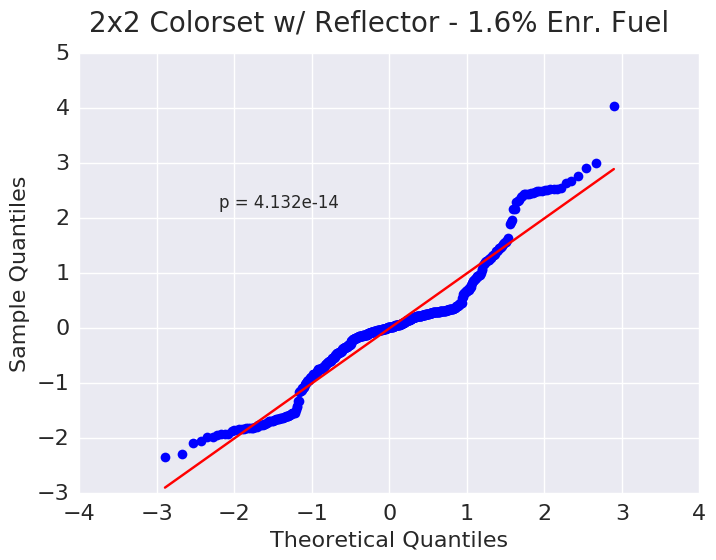
\includegraphics[width=\linewidth]{figures/patterns/reflector/quantile/16-enr-fiss-2}  \caption{}
  \label{fig:chap9-qq-reflector-1.6-fiss}
\end{subfigure}
\begin{subfigure}{0.5\textwidth}
  \centering
  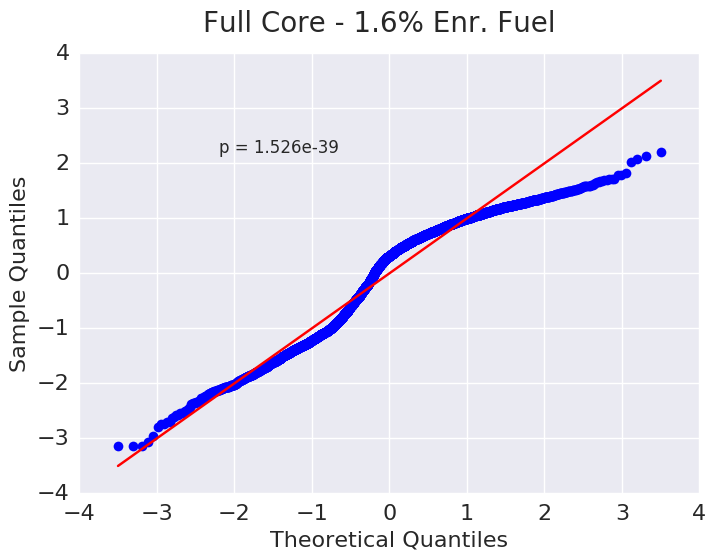
\includegraphics[width=\linewidth]{figures/patterns/full-core/quantile/16-enr-fiss-2} \caption{}
  \label{fig:chap9-qq-full-core-1.6-fiss}
\end{subfigure}
\caption[Q-Q plots of U-235 fission MGXS for 1.6\% enriched fuel]{\ac{Q-Q} plots of U-235 fission \ac{MGXS} (group 2 of 2) for 1.6\% enriched fuel.}
\label{fig:chap9-qq-1.6-fiss}
\end{figure}

\begin{figure}[h!]
\centering
\begin{subfigure}{0.5\textwidth}
  \centering
  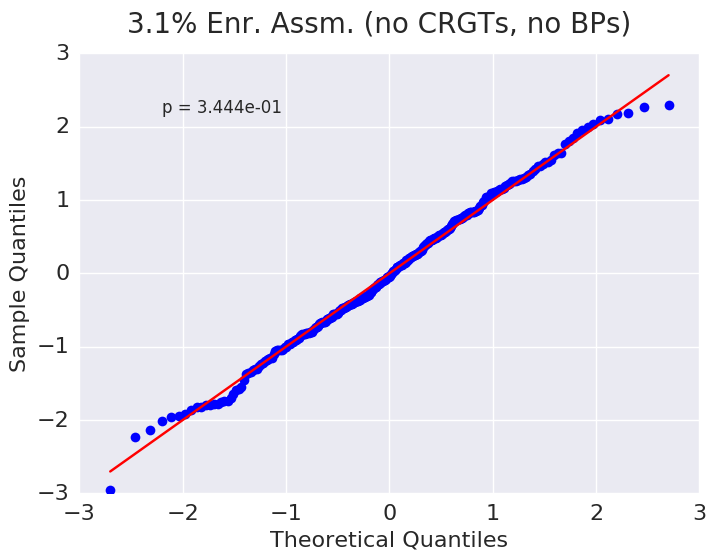
\includegraphics[width=\linewidth]{figures/patterns/assm-3.1-inf/quantile/assm-31-inf-fiss-2}
  \caption{}
  \label{fig:chap9-qq-assm-3.1-inf-fiss}
\end{subfigure}%
\begin{subfigure}{0.5\textwidth}
  \centering
  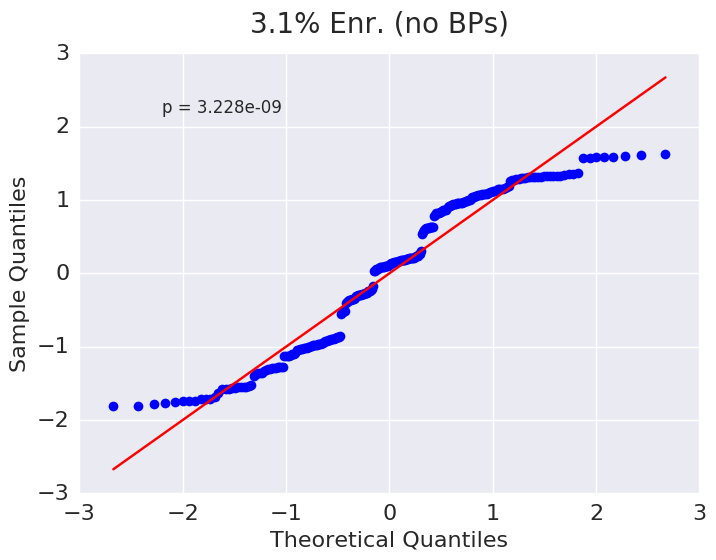
\includegraphics[width=\linewidth]{figures/patterns/assm-3.1/quantile/assm-31-fiss-2}
  \caption{}
  \label{fig:chap9-qq-assm-3.1-fiss}
\end{subfigure}
\begin{subfigure}{0.5\textwidth}
  \centering
  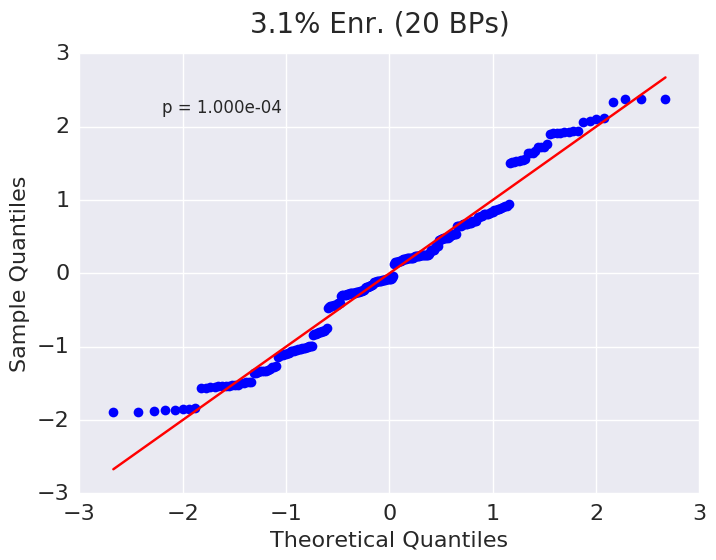
\includegraphics[width=\linewidth]{figures/patterns/assm-3.1-20BPs/quantile/assm-31-20BPs-fiss-2}
  \caption{}
  \label{fig:chap9-qq-assm-3.1-20BPs-fiss}
\end{subfigure}%
\begin{subfigure}{0.5\textwidth}
  \centering
  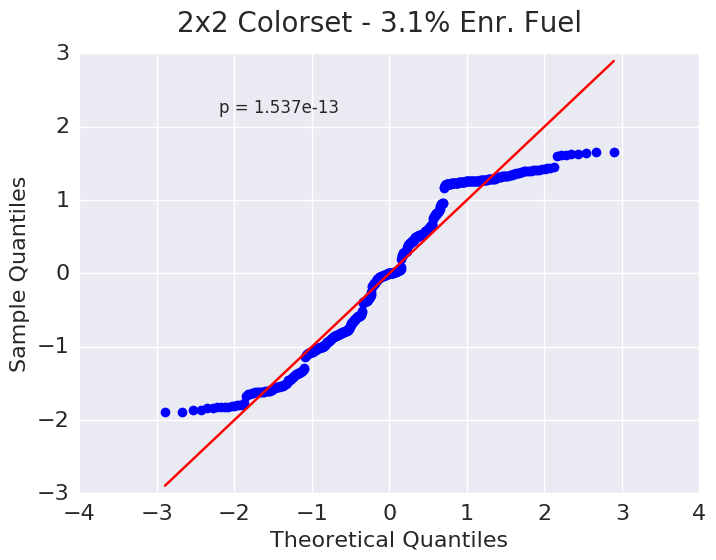
\includegraphics[width=\linewidth]{figures/patterns/2x2/quantile/31-enr-fiss-2}
  \caption{}
  \label{fig:chap9-qq-2x2-3.1-fiss}
\end{subfigure}
\begin{subfigure}{0.5\textwidth}
  \centering
  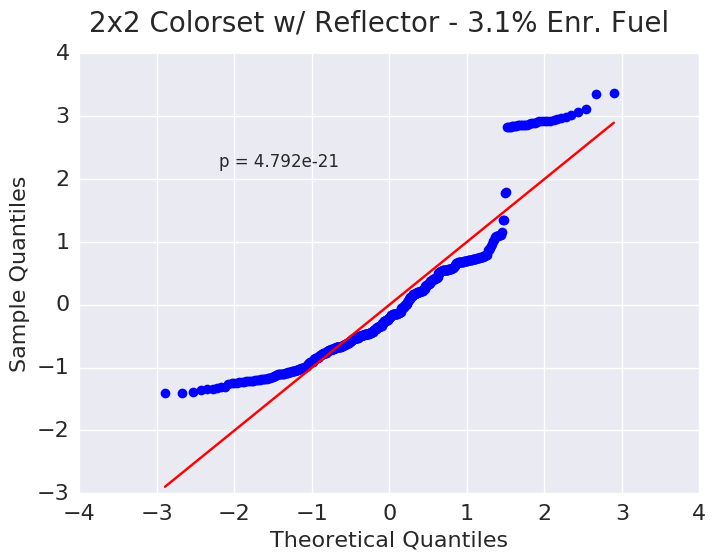
\includegraphics[width=\linewidth]{figures/patterns/reflector/quantile/31-enr-fiss-2}  \caption{}
  \label{fig:chap9-qq-reflector-3.1-fiss}
\end{subfigure}%
\begin{subfigure}{0.5\textwidth}
  \centering
  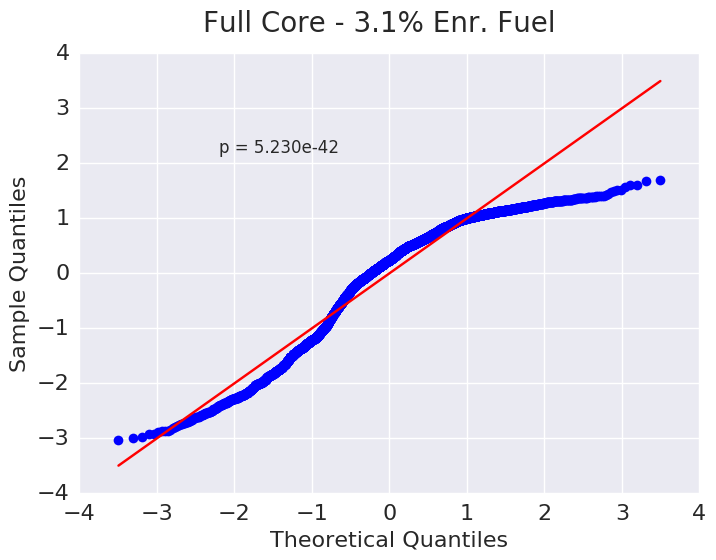
\includegraphics[width=\linewidth]{figures/patterns/full-core/quantile/31-enr-fiss-2} \caption{}
  \label{fig:chap9-qq-full-core-3.1-fiss}
\end{subfigure}
\caption[Q-Q plots of U-235 fission MGXS 3.1\% enriched fuel]{\ac{Q-Q} plots of U-235 fission \ac{MGXS} (group 2 of 2) for 3.1\% enriched fuel.}
\label{fig:chap9-qq-3.1-fiss}
\end{figure}

As was observed in the preceding section for U-238 capture, the datasets for the infinite lattices in Figs.~\ref{fig:chap9-qq-assm-1.6-inf-fiss} and~\ref{fig:chap9-qq-assm-3.1-inf-fiss} appear to be from a normal distribution since they lie very close to the $y = x$ reference line. In addition, the $p$-values are greater than 0.3, well above commonly used significance levels; thus one would not reject the null hypothesis that the data is from a normal distribution. The addition of \acp{CRGT} leads to a clear deviation from normality in Figs.~\ref{fig:chap9-qq-assm-1.6-fiss} and~\ref{fig:chap9-qq-assm-3.1-fiss}. However, the structure is substantially more complex than the four shoulders exhibited in the U-238 capture \ac{MGXS} data. As was noted in Sec.~\ref{subsubsec:chap9-histograms-fiss}, the presence of \acp{BP} results in many distinct clusters which appear as a highly fragmented, steplike profile in the \ac{Q-Q} plot in Fig.~\ref{fig:chap9-qq-assm-3.1-20BPs-capt}. The high degree of clustering exhibited in the histograms and rug plots for the larger colorset and quarter core benchmarks similarly appears in the corresponding \ac{Q-Q} plots.

As noted for the U-238 capture \ac{MGXS}, the $p$-values for the Shapiro-Wilks tests of the pin-wise U-235 fission \ac{MGXS} data affirm the deviation from normality seen in the \ac{Q-Q} plots. Of particular note, $p$-values on the order of 10$^{-39}$ and 10$^{-44}$ arise from the data for the 1.6\% and 3.1\% enriched fuel pins, respectively, for the \ac{BEAVRS} quarter core model. These results suggest that it is highly unlikely that the data arose from a normally distributed stochastic process.

%-mention that tails above and below on lower/upper range indicate that tails of distribution are not as wide as would be expected for normal samples -- e.g., a ``tighter'' or ``narrower'' distribution
%-3.1\% enr pins in full core are tighter on bottom edge, but wider on upper edge
%  -indicative of those few ``outlier'' pins with \ac{MGXS} near 0.9 barns in Fig.~\ref{fig:chap9-hist-3.1-capt}

\begin{emphbox}
\textbf{The higher degree of clustering of pin-wise U-235 fission \ac{MGXS} than U-238 capture \ac{MGXS} results in highly fragmented steplike \ac{Q-Q} plots. The Shapiro-Wilks test once again rejects the null hypothesis that the \ac{MGXS} data is drawn from a normal distribution for all six heterogeneous benchmarks.}
\end{emphbox}


%%%%%%%%%%%%%%%%%%%%%%%%%%%%%%%%%%%%%%%%%%%%%%%%%%%%%%%%%%%%%%%%%%%%%%%%%%%%%%%
\section{LNS Spatial Homogenization}
\label{sec:chap9-lns-homogenize}

The preceding sections quantified and visualized the dispersion and structural clustering of pin-wise \ac{MGXS} due to spatial self-shielding effects. The degenerate spatial homogenization scheme evaluated in Chap.~\ref{chap:quantify} is able to model the clustering of \ac{MGXS} by assigning a unique set of \ac{MGXS} to each fuel pin instance in a core geometry. However, the infinite and null schemes fail to account for \ac{MGXS} clustering since they each assign a single \ac{MGXS} to all instances of the same fuel pin type. As evidenced by the results in Chap.~\ref{chap:quantify}, it is important to adequately model clusters of pin-wise \ac{MGXS} in order to accurately predict U-238 capture rate spatial distributions. 

This section introduces a new spatial homogenization scheme which use a deterministic  approach to cluster pin-wise \ac{MGXS} based on an analysis of the core geometry. The approach developed here is akin to geometric templates employed by some commonly used lattice physics codes, such as CASMO~\cite{rhodes2006casmo}, to predict which groupings of pins are likely to experience similar spatial self-shielding effects and hence have similar microscopic \ac{MGXS}. The new scheme is termed \textit{\ac{LNS} homogenization} since it is predicated upon OpenCG's Local Neighbor Symmetry (LNS) algorithm (see Sec.~\ref{sec:chap4-lns}). The \ac{LNS} algorithm analyzes the combinatorial geometry (CG) used to represent each benchmark model and groups pins together based on their neighboring spatial zones. The goal of \ac{LNS} homogenization is to achieve degenerate homogenization's predictive accuracy by representing \ac{MGXS} clustering, and approach null homogenization's tally convergence rate by averaging \ac{MGXS} across many pin instances.

%%%%%%%%%%%%%%%%%%%%%
\subsection{Overview}
\label{sec:chap9-lns-overview}

Like the degenerate spatial homogenization scheme (Sec.~\ref{subsec:chap8-degenerate}), a single \ac{MC} calculation of the complete heterogeneous geometry is used to generate \ac{MGXS} for all materials. The \ac{MGXS} are tallied separately for each instance of fissile material zones using OpenMC's distributed cell tallies (see Sec.~\ref{subsec:chap4-distribcells}). The OpenCG \ac{LNS} algorithm assigns an integral \ac{LNS} identifier to each unique pin instance in the \ac{CG} based on an analysis of each pin's neighbors at each level of the \ac{CG} hierarchy. Pins with like neighboring pins, within assemblies with like neighboring assemblies, will receive the same \ac{LNS} identifier\footnote{\ac{LNS} hashes a data structure representing a rotationally invariant form of each pin's neighbors.}. The \ac{MGXS} are averaged across all pin instances with the same unique \ac{LNS} identifier. For example, all pins adjacent to a single \ac{CRGT} on one face and fuel pins on all other faces are assigned the same \ac{MGXS} averaged across the OpenMC distributed cell tallies for all of those pin instances. The OpenCG region differentiation algorithm (see Sec.~\ref{sec:chap4-region-diff}) is used to build an OpenMOC geometry with unique cells and materials for each fuel pin which mirrors the \ac{LNS} representation of the \ac{CG} model. Like the infinite, null and degenerate schemes, spatial self-shielding effects experienced by different non-fissile spatial zones are averaged across the entire geometry for each non-fissile material.

The total number of materials (\textit{i.e.}, \ac{MGXS}) used to model each benchmark with each homogenization scheme is given in Tab.~\ref{fig:chap9-lns-materials}. The fuel assemblies with \acp{CRGT} and \acp{BP} and 2$\times$2 colorset benchmark models are color-coded by material and illustrated in Fig.~\ref{fig:chap9-lns-materials} for the \ac{LNS} homogenization scheme. Likewise, the materials for the quarter core \ac{BEAVRS} model with \ac{LNS} homogenization is highlighted in Fig.~\ref{fig:chap9-lns-materials-beavrs}. 

\begin{table}[h!]
  \centering
  \caption[Number of materials for LNS spatial homogenization]{Number of materials modeled with unique \ac{MGXS} in each heterogeneous benchmark for \ac{LNS} spatial homogenization.}
  \small
  \label{table:chap9-num-materials-lns}
  \vspace{6pt}
  \begin{tabular}{l r r r}
  \toprule
  \rowcolor{lightgray}
  & \multicolumn{3}{c}{\cellcolor{lightgray} \bf \# Materials} \\
  \multirow{-2}{*}{\cellcolor{lightgray} \bf Benchmark} &
  \multicolumn{1}{c}{\cellcolor{lightgray} \bf Null/Infinite} &
  \multicolumn{1}{c}{\cellcolor{lightgray} \bf \ac{LNS}} &
  \multicolumn{1}{c}{\cellcolor{lightgray} \bf Degenerate} \\
  \midrule
1.6\% Assm & 5 & 13 & 268 \\
  \midrule
3.1\% Assm & 5 & 13 & 268 \\
  \midrule
3.1\% Assm w/ 20 BPs & 7 & 17 & 270  \\
  \midrule
2$\times$2 Colorset & 8 & 25 & 1,062 \\
  \midrule
2$\times$2 Colorset w/ Reflector & 8 & 35 & 1,062 \\
  \midrule
\ac{BEAVRS} Quarter Core & 10 & 502 & 13,000 \\ % LNS = ceil(193 / 4) * 10 + 7 - actually just counted them up as 10 for assms with BPs and 8 otherwise
  \bottomrule
\end{tabular}
\end{table}

\begin{figure}[h!]
\centering
\begin{subfigure}{.45\textwidth}
  \centering
  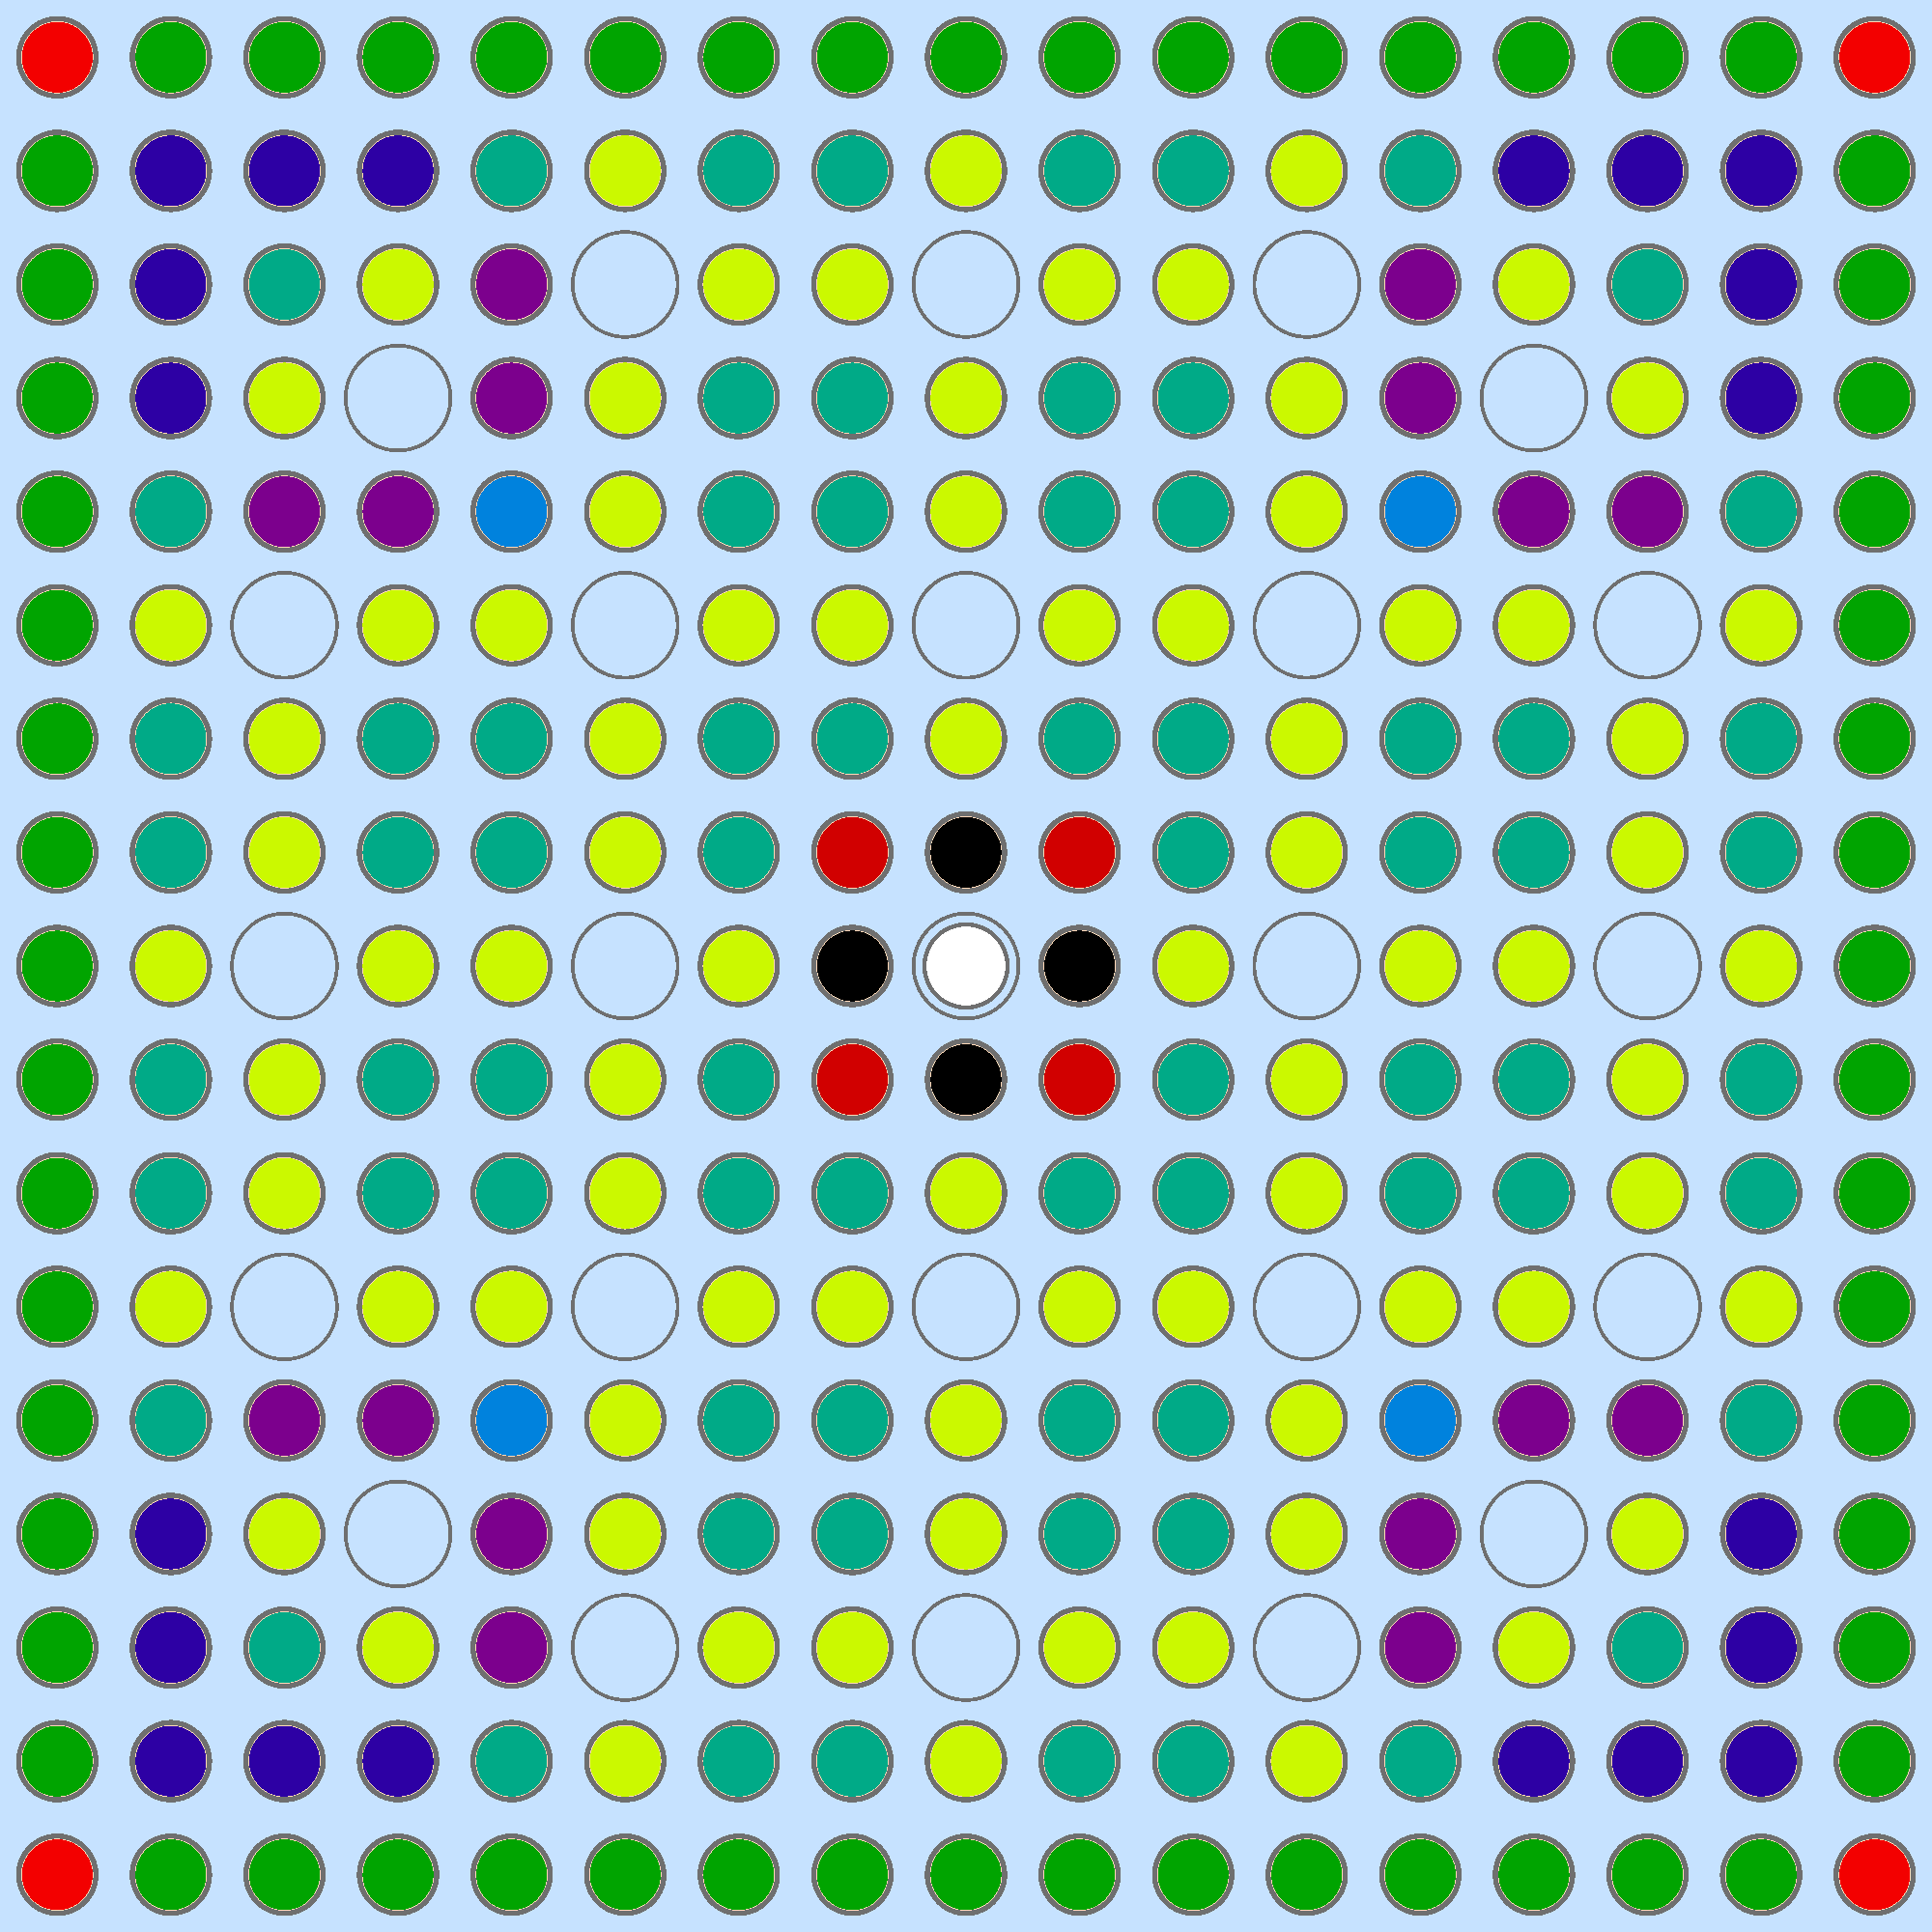
\includegraphics[width=0.9\linewidth]{figures/patterns/lns/assm-31/materials}
  \caption{}
  \label{fig:chap9-assm-31-lns-materials}
\end{subfigure}%
\begin{subfigure}{.45\textwidth}
  \centering
  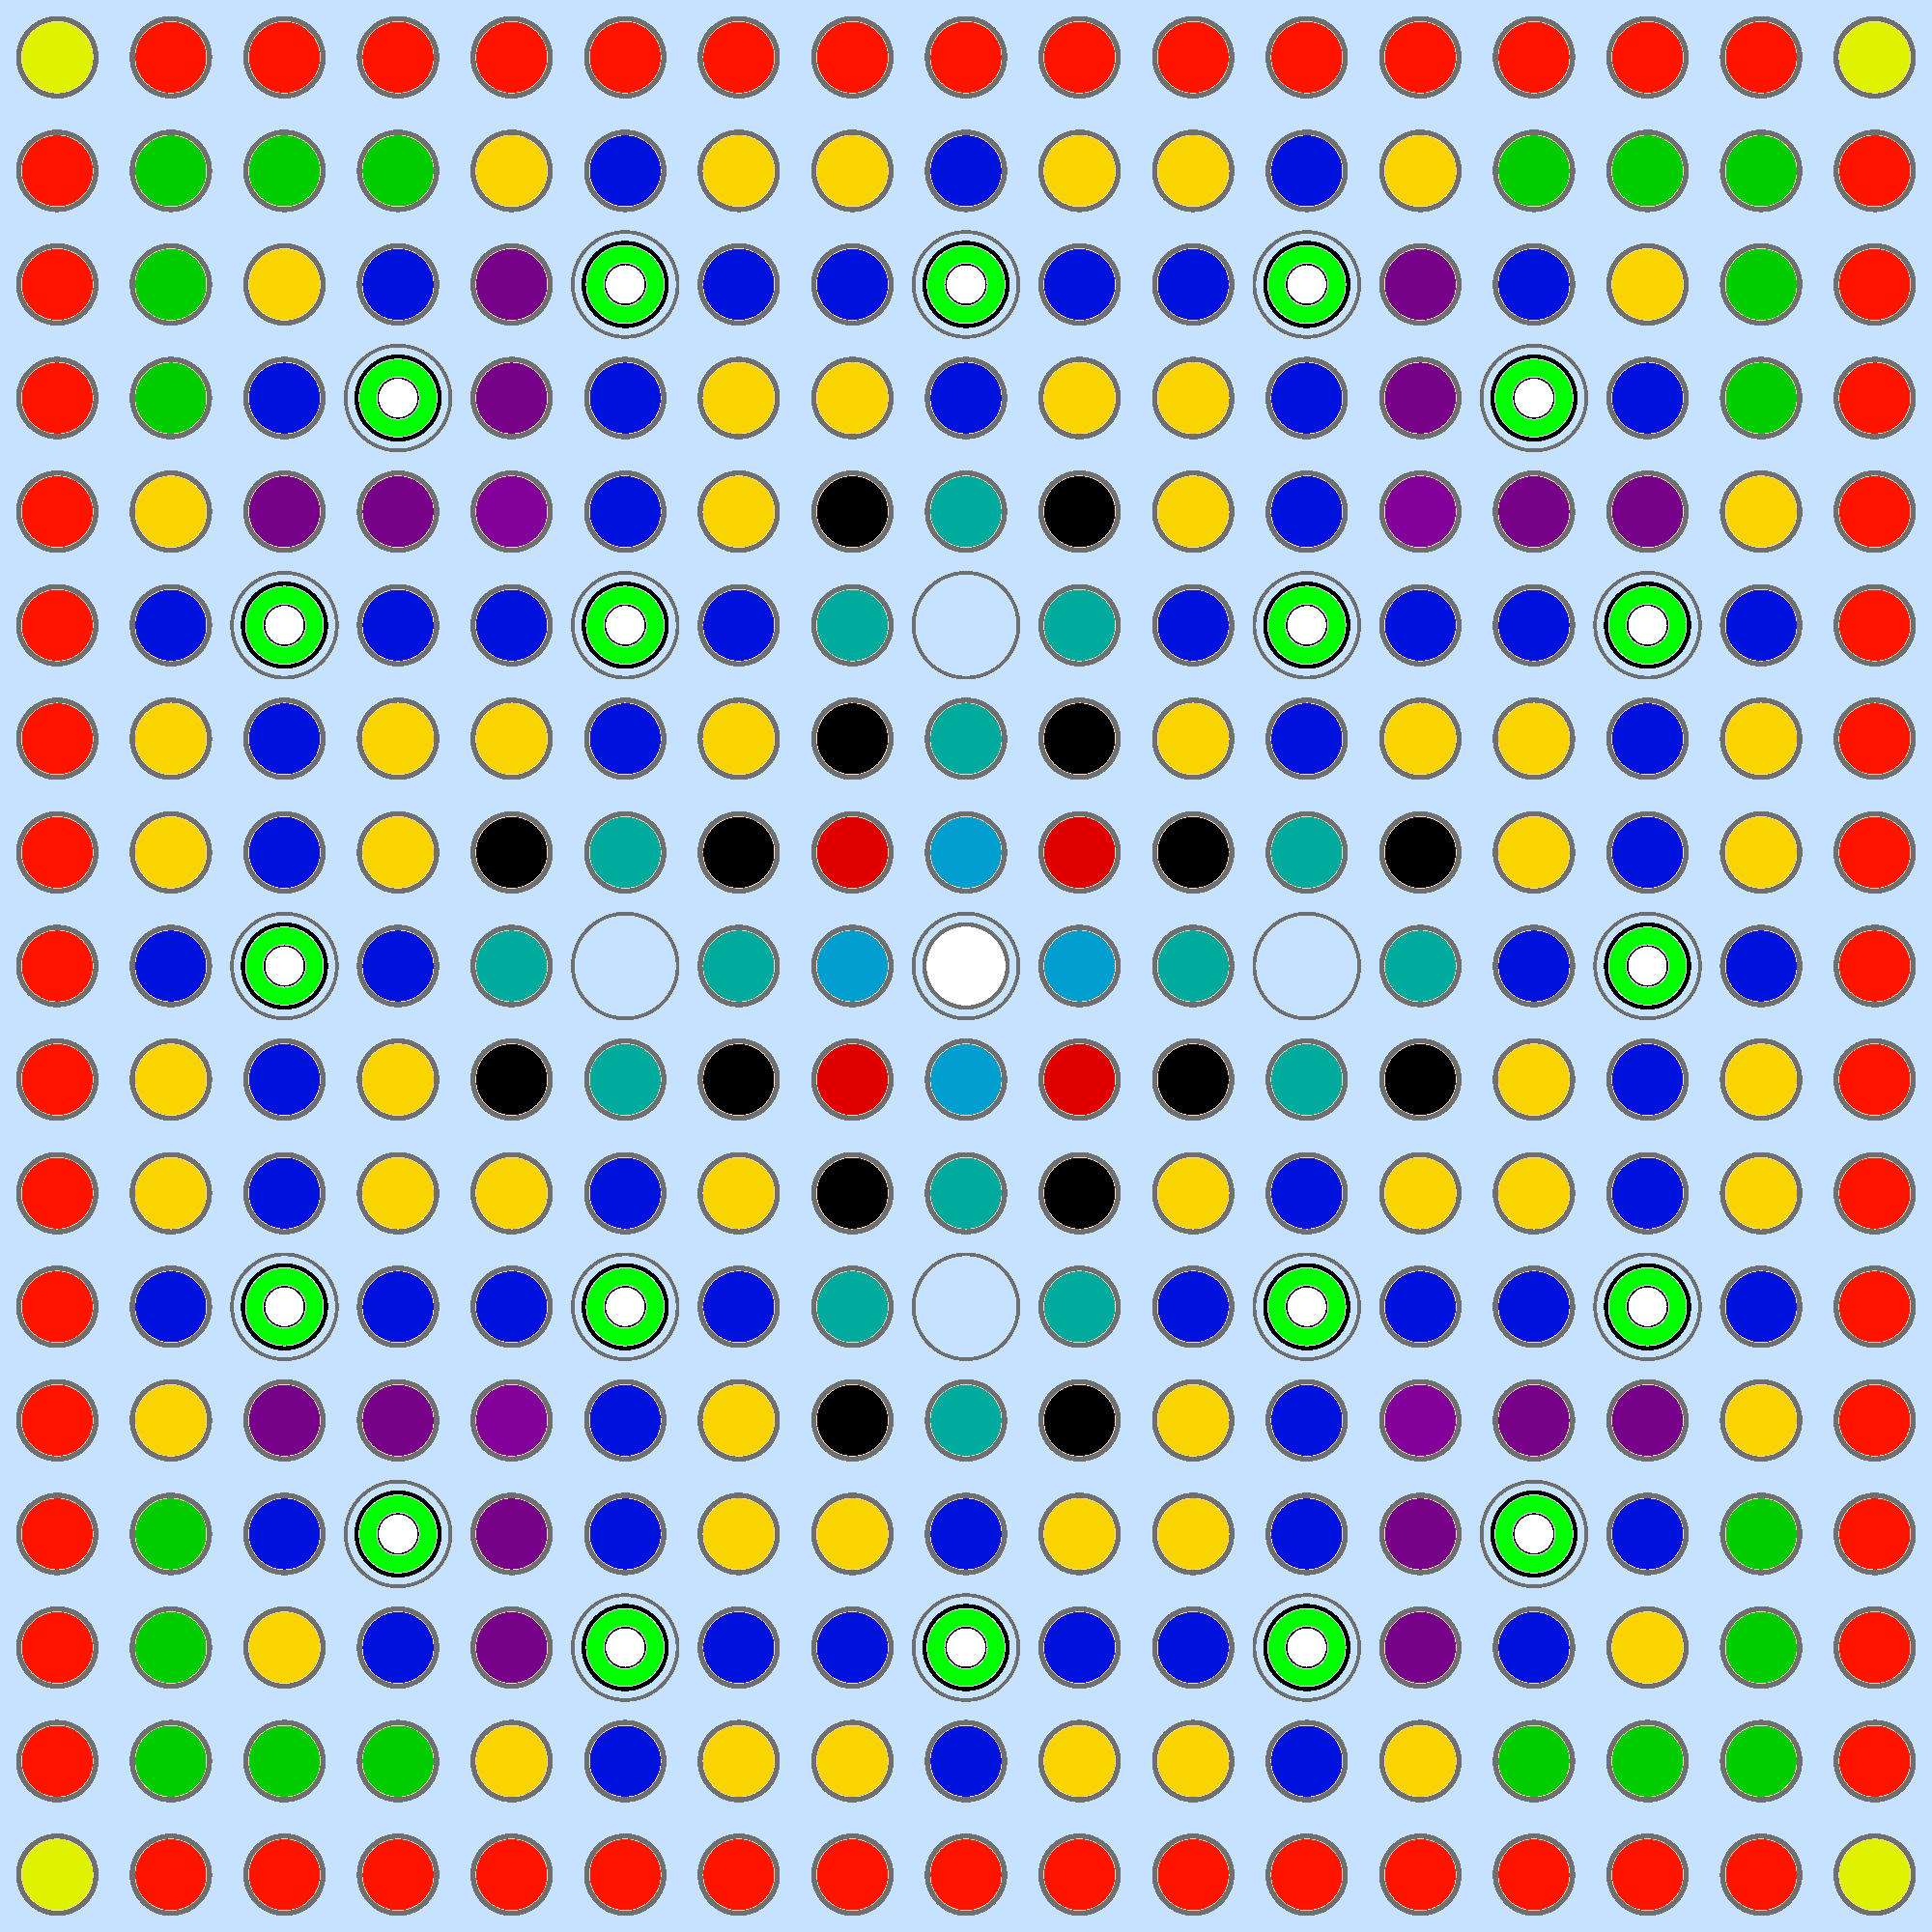
\includegraphics[width=0.9\linewidth]{figures/patterns/lns/assm-31-20BPs/materials}
  \caption{}
  \label{fig:chap9-31-20BPs-lns-materials}
\end{subfigure}
\begin{subfigure}{.45\textwidth}
  \centering
  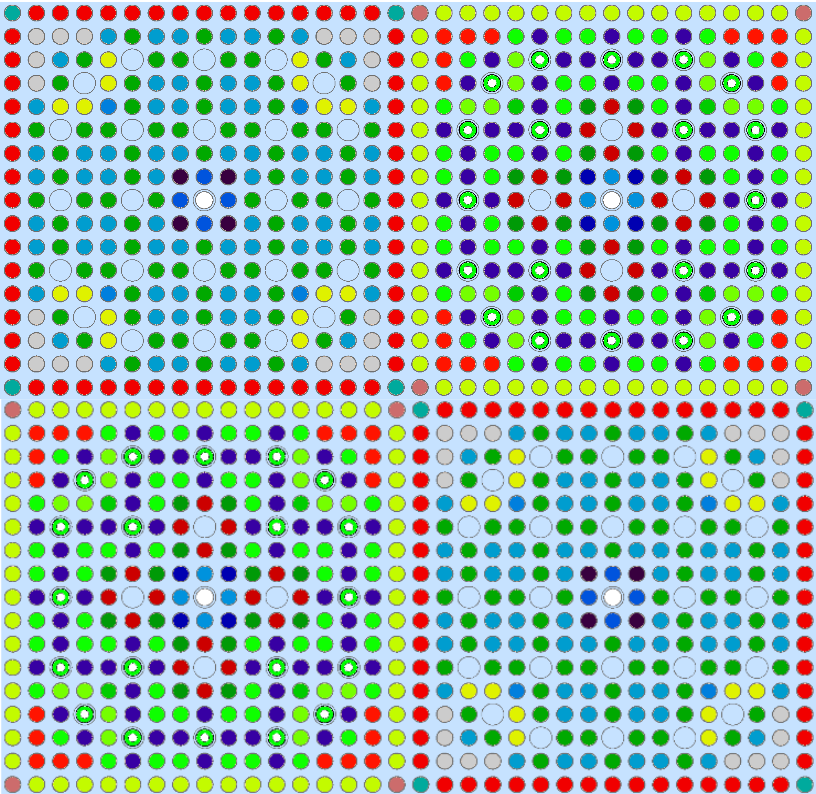
\includegraphics[width=0.9\linewidth]{figures/patterns/lns/2x2/materials}
  \caption{}
  \label{fig:chap9-2x2-lns-materials}
\end{subfigure}%
\begin{subfigure}{.45\textwidth}
  \centering
  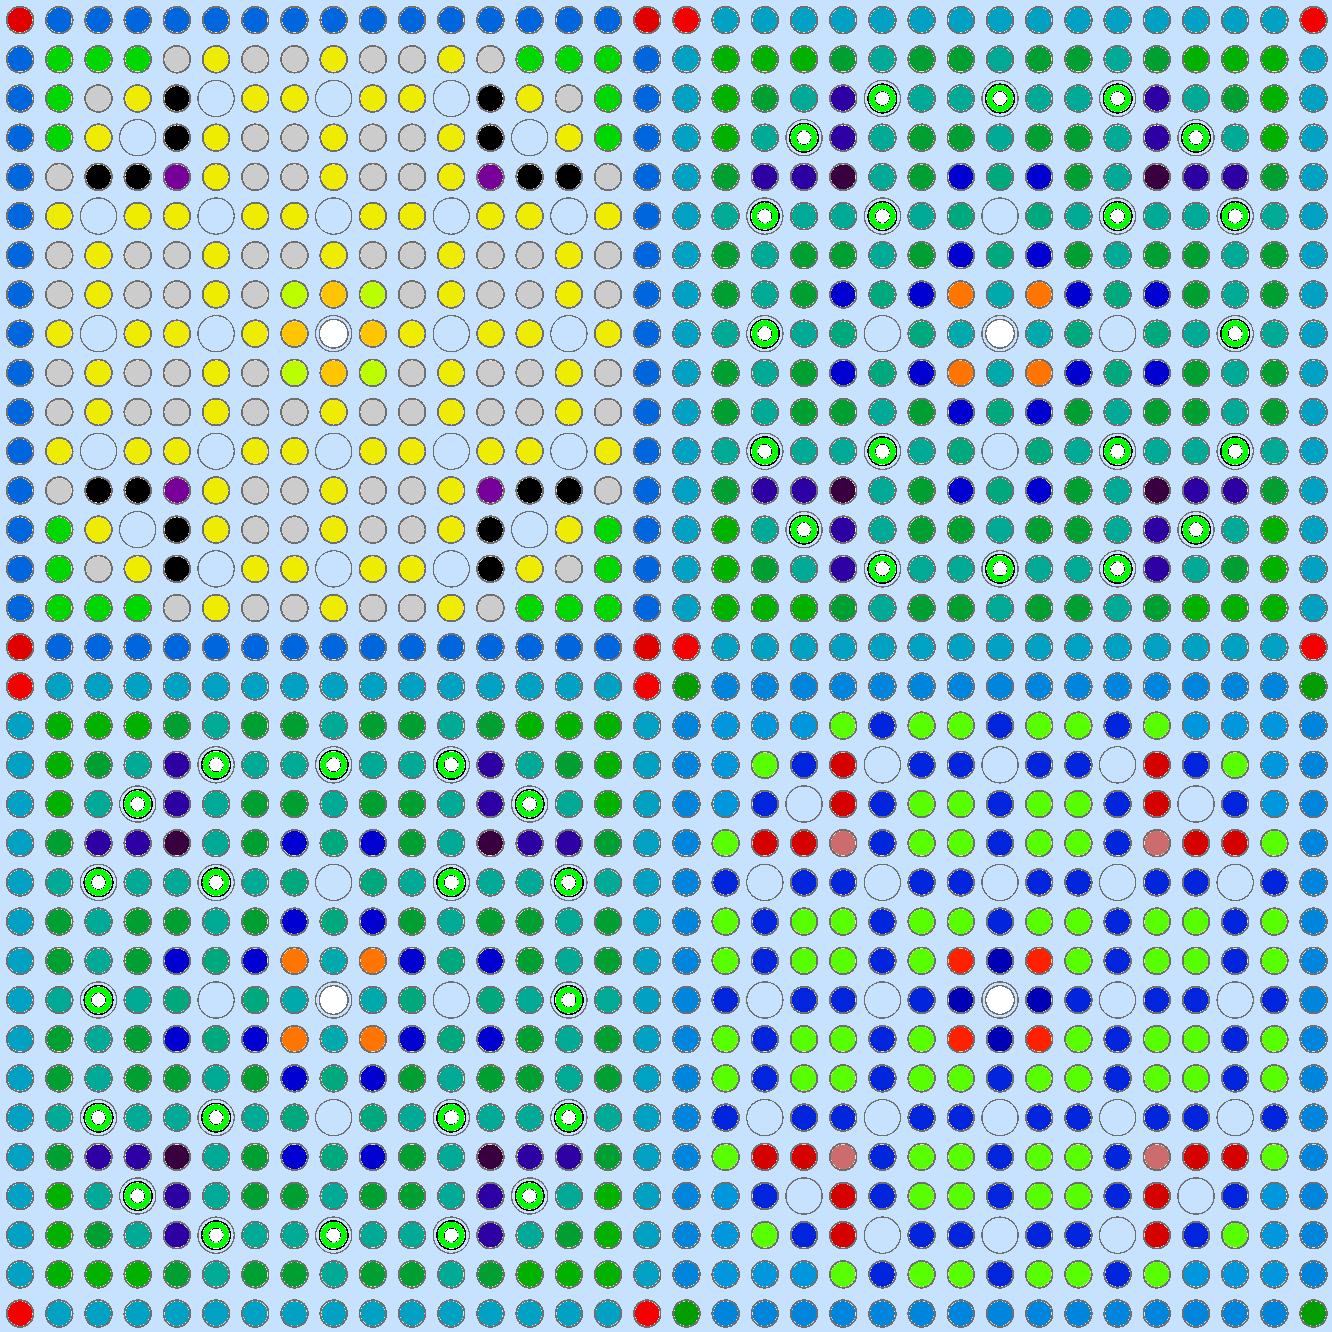
\includegraphics[width=0.9\linewidth]{figures/patterns/lns/reflector/materials}
  \caption{}
  \label{fig:chap9-reflector-lns-materials}
\end{subfigure}
\caption[Depiction of LNS spatially homogenized materials]{OpenMOC materials with \ac{LNS} spatial homogenization for an assembly with \acp{CRGT} (a), an assembly with 20 \acp{BP} (b), a 2$\times$2 colorset without (c) and with (d) a reflector. Each uniquely colored material represents a unique set of \ac{MGXS}.}
\label{fig:chap9-lns-materials}
\end{figure}

\begin{figure}[h!]
\centering
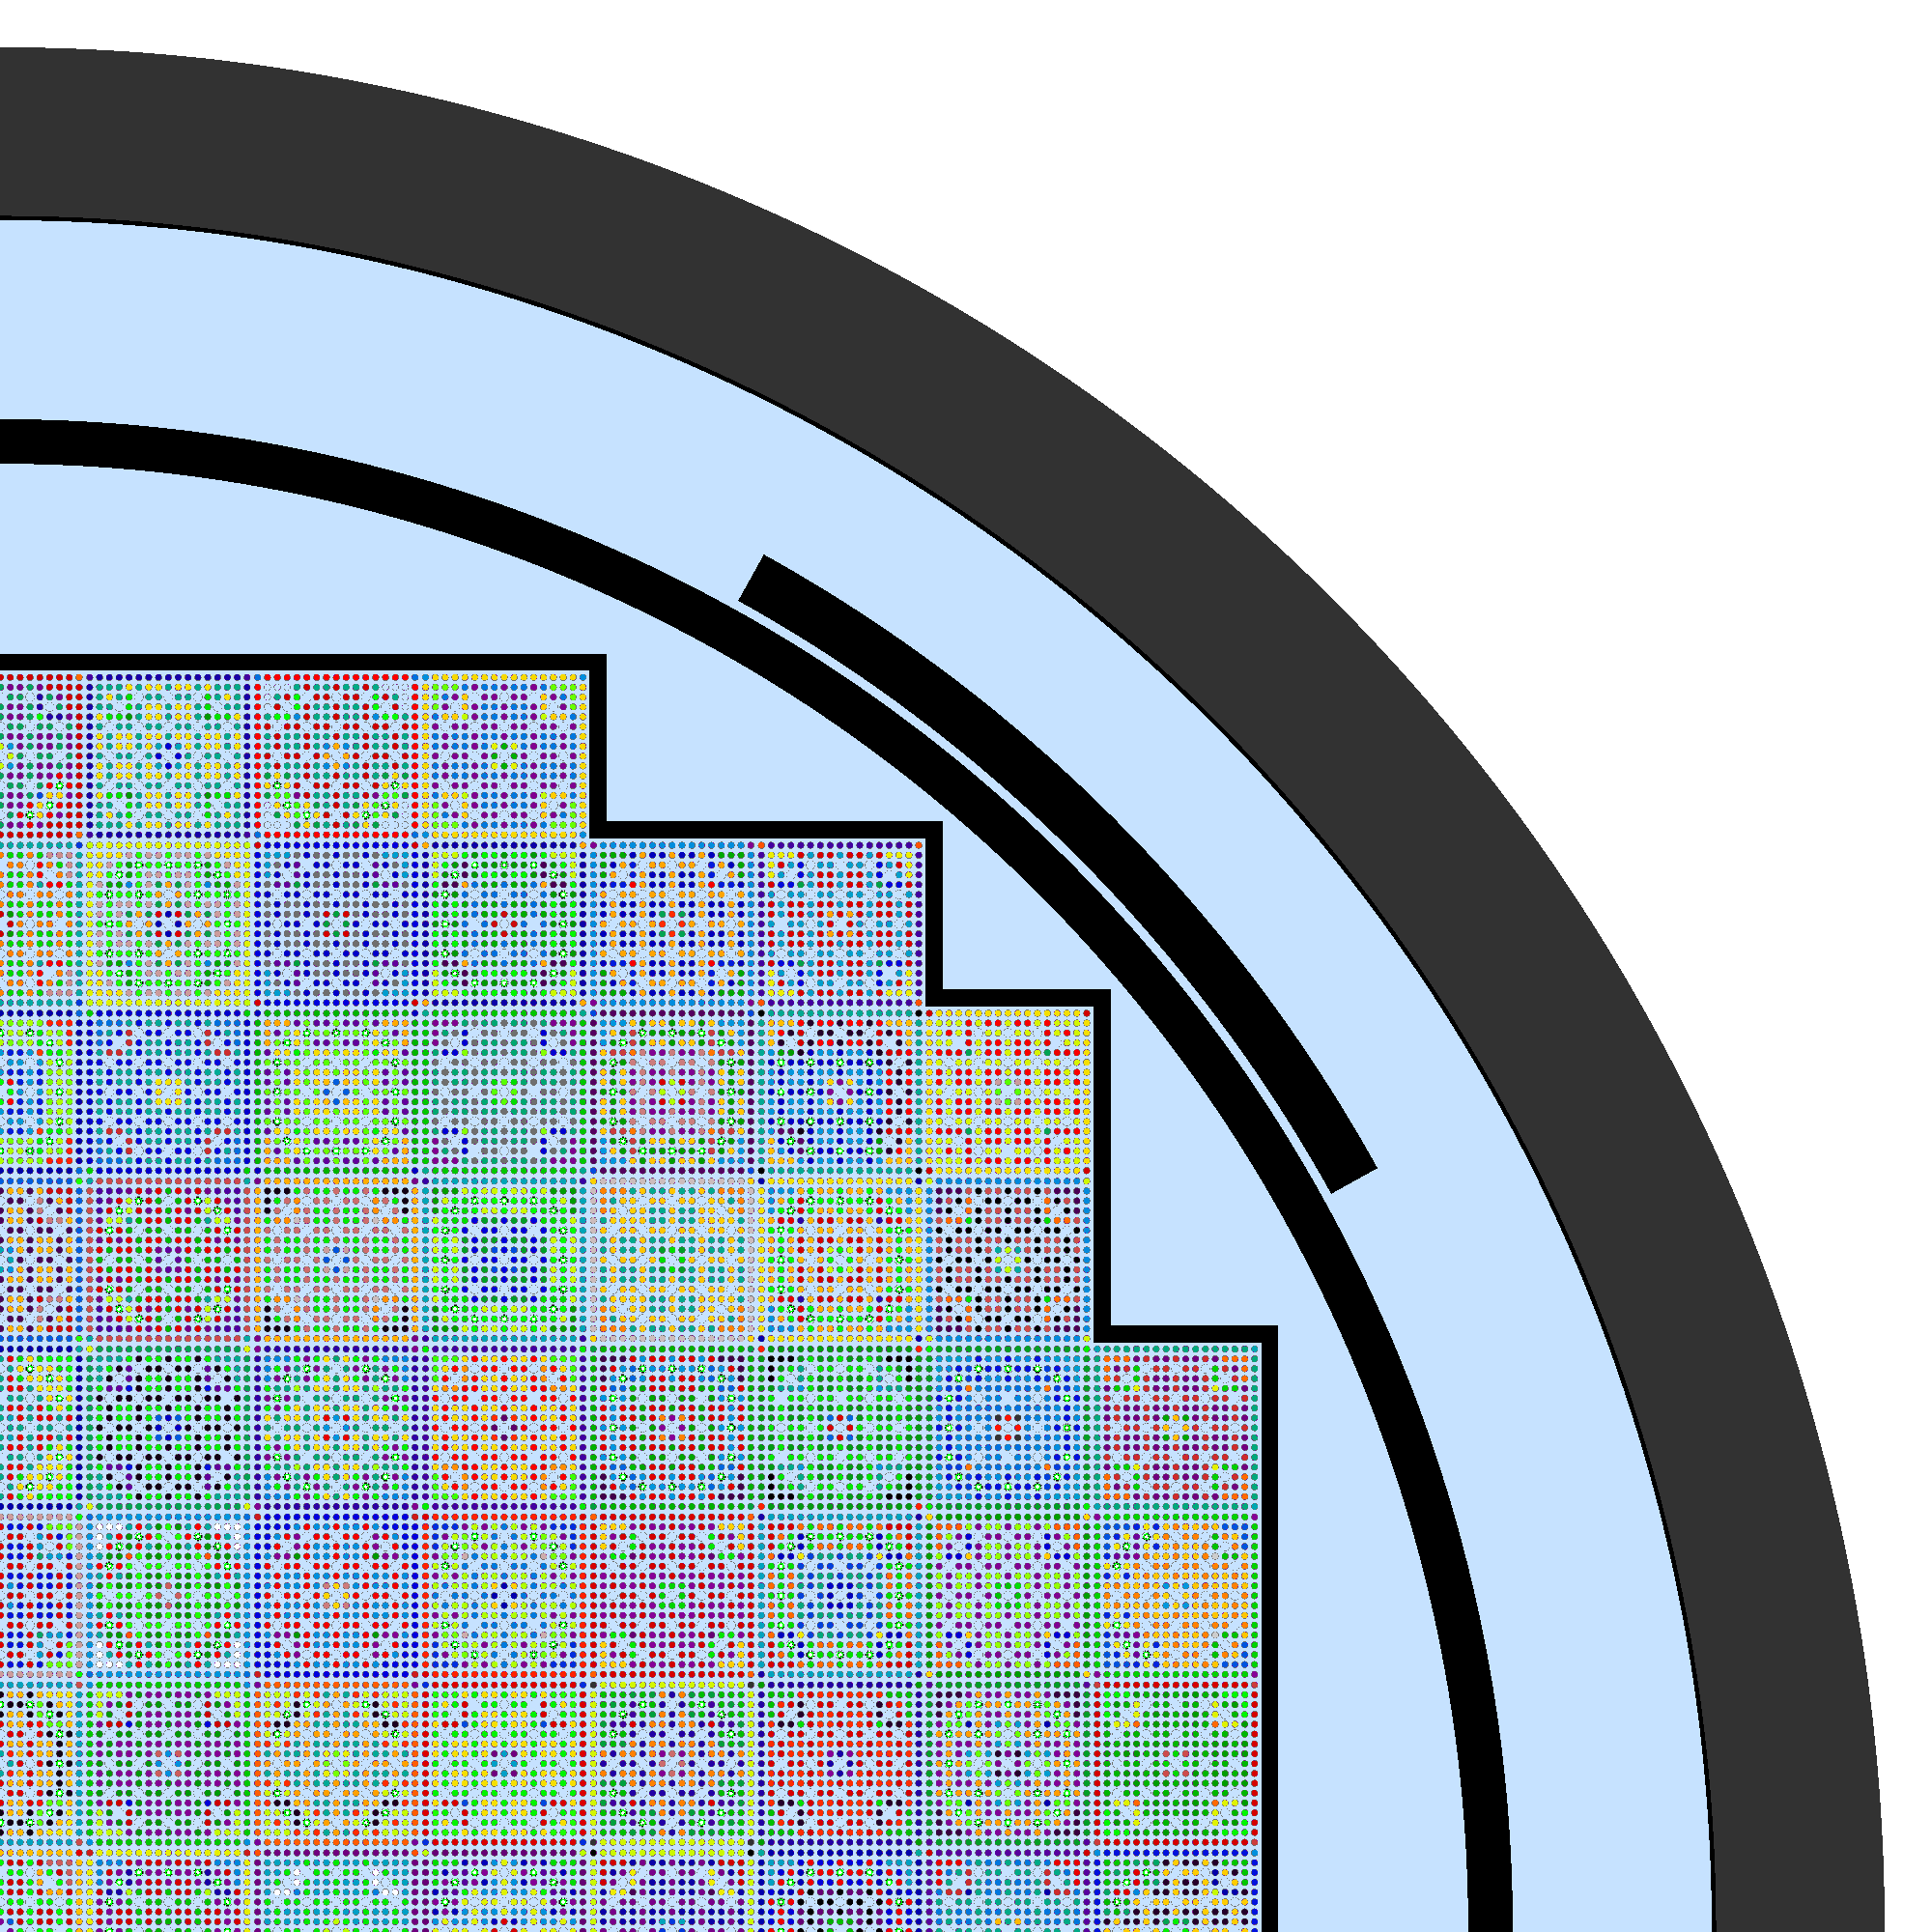
\includegraphics[width=\linewidth]{figures/patterns/lns/full-core/materials}
\vspace{2mm}
\caption[Depiction of LNS spatially homogenized materials for BEAVRS]{OpenMOC materials with \ac{LNS} spatial homogenization for the 2D quarter core \ac{BEAVRS} model. Each uniquely colored material represents a unique set of \ac{MGXS}.}
\label{fig:chap9-lns-materials-beavrs}
\end{figure}

As quantified in the Tab.~\ref{table:chap9-num-materials-lns}, 8 -- 10 unique fissile materials are used for each fuel assembly with \ac{LNS}, far fewer than the 264 in degenerate homogenization. Consequently, the \ac{MC} tallies for \ac{LNS} homogenization will ``converge'' much more quickly than those for degenerate homogenization. In addition, as indicated by the figures, fuel pin types with neighboring heterogeneities are assigned unique \ac{MGXS} which generally reflect the clustering of \ac{MGXS} due to spatial self-shielding effects. As a result, \ac{LNS} homogenization would be expected to predict reaction rate distributions better than the null scheme. 

%%%%%%%%%%%%%%%%%%%%%%%%%%%%%%%%%%%%%%%%
\subsection{Track Density-Weighted MGXS}
\label{sec:chap9-lns-math}

The \ac{LNS} spatially-homogenized \ac{MGXS} for each group of pin instances are not simply computed as the geometric average of the \ac{MGXS} in each pin instance. Instead, the total reaction rates and fluxes in each pin instance are first summed together and then divided to compute an average \ac{MGXS} which is effectively weighted by the relative particle track density in each fuel pin instance. The track density-weighted average \ac{MGXS} preserve global reaction rates\footnote{A simple geometric average of \ac{MGXS} across fuel pins will not preserve global reaction rates.} and are equivalent to defining specialized OpenMC ``cell'' reaction rate and flux tallies for each group of pin instances with like \ac{LNS} identifiers. 

In order to formally express the track density weighted-average approach, it is useful to first recall Eqn.~\ref{eqn:chap3-general-micro} for a microscopic \ac{MGXS} estimated from \ac{MC} tallies for reaction $x$, nuclide $i$, spatial zone $k$ and energy group $g$:

\begin{equation}
\label{eqn:chap9-general-micro}
\hat{\sigma}_{x,i,k,g} = \frac{\langle \sigma_{x,i}, \psi \rangle_{k,g}^{t\ell}}{\langle \psi \rangle_{k,g}^{t\ell}}
\end{equation}

\noindent In this context, the index $k$ of $K$ total spatial zones refers to a particular instance of a fuel pin within a core geometry. The \ac{LNS} algorithm represents a function $S(k)$ which assigns an identifier $m$ to each fuel pin instance based on its neighbors (\textit{i.e.}, pin instances with the same neighbors are assigned the same identifier). The set $\mathbb{S}_{m}$ encapsulates all instances $k$  with the same \ac{LNS} identifier:

\begin{equation}
\label{eqn:chap9-lns-set}
\mathbb{S}_{m} = \left\{1 \le k \le K: S(k) = m\right\}
\end{equation}

\ac{LNS} homogenization computes a single set of \ac{MGXS} for the fuel pin instances in each set $k \in \mathbb{S}_{m}$ classified by the \ac{LNS} algorithm. This is equivalent to a specialization of Eqn.~\ref{eqn:chap9-general-micro} with track density-weighted averages of the reaction rates and flux tallies in each pin instance:

\begin{equation}
\label{eqn:chap9-lns-micro}
\hat{\sigma}_{x,i,m,g} = \frac{\displaystyle\sum\limits_{k=1}^{K}\mathbb{1}_{\mathbb{S}_{m}}(k) \langle \sigma_{x,i}, \psi \rangle_{k,g}^{t\ell}}{\displaystyle\sum\limits_{k=1}^{K}\mathbb{1}_{\mathbb{S}_{m}}(k) \langle \psi \rangle_{k,g}^{t\ell}}
\end{equation}

\noindent where the indicator function $\mathbb{1}_{\mathbb{S}_{m}}(k)$ is equal to 1 if $k \in \mathbb{S}_{m}$ and 0 otherwise. The track density-weighted average is similarly applied to the \ac{MC} tallies for each type of \ac{MGXS}, including scattering matrices and the fission spectrum.

%%%%%%%%%%%%%%%%%%%%%%%%%%%%%%%%%%%%%%%%
\subsection{Potential Shortcomings}
\label{sec:chap9-lns-shortcomings}

Upon further inspection, it is clear from Figs.\ref{fig:chap9-lns-materials} and~\ref{fig:chap9-lns-materials-beavrs} that there are some notable shortcomings to the \ac{LNS} scheme. For example, the pins along the inter-assembly and assembly-reflector interfaces in the 2$\times$2 colorset and quarter core \ac{BEAVRS} models in Fig.~\Crefrange{fig:chap9-2x2-lns-materials}{fig:chap9-reflector-lns-materials} and~\ref{fig:chap9-lns-materials-beavrs} are treated the same (\textit{i.e.}, with the same \ac{MGXS}). As a result, \ac{LNS} may result in poor reaction rate predictions for these pins, as will be quantified in Sec.~\ref{sec:chap9-lns-results}. It is possible that the \ac{LNS} algorithm could be specialized in various ways to differentiate between the pin types on the outer edge of each assembly. However, such customizations would not be reactor agnostic and would be challenging to implement and generalize.

Furthermore, the relative number of \ac{LNS} materials does not scale with the total number of fuel pins. In particular, there are 26 -- 33$\times$ fewer materials with the \ac{LNS} scheme as compared to the degenerate scheme for the individual fuel assembly benchmarks as well as the quarter core \ac{BEAVRS} model\footnote{This reflects the fact that neighboring assemblies are accounted for in the \ac{LNS} algorithm. The fuel assemblies in the quarter core \ac{BEAVRS} model do not exhibit any neighboring symmetries, and as a result, no two assemblies are assigned the same set of pin-wise \ac{MGXS}.}. It is likely that \ac{LNS} uses more materials than necessary to capture \ac{MGXS} clustering for large geometries, which will diminish its relative accelerated convergence rate with respect to degenerate homogenization.

\begin{emphbox}
\textbf{\ac{LNS} spatial homogenization applies a ``geometric template'' to homogenize \ac{MGXS} for pins with similar neighboring spatial zones. The scheme aims to improve the \ac{MC} tally convergence rate while capturing spatial self-shielding effects in clustered \ac{MGXS}. However, the number of materials scales poorly with the size and complexity of the core geometry. Furthermore, the algorithm fails to distinguish pins with very different spatial self-shielding effects at inter-assembly and assembly-reflector interfaces.}
\end{emphbox}


%%%%%%%%%%%%%%%%%%%%%%%%%%%%%%%%%%%%%%%%%%%%%%%%%%%%%%%%%%%%%%%%%%%%%%%%%%%%%%%%
\section{Multi-Group Results with LNS}
\label{sec:chap9-lns-results}

Each of the six benchmarks was modeled with OpenMOC using \ac{MGXS} generated by the \ac{LNS} spatial homogenization scheme. Each of the six heterogeneous benchmarks was modeled with 2-, 8- and 70-group \ac{MGXS} using the same OpenMOC runtime parameters as those used in Chap.~\ref{chap:quantify} for infinite, null and degenerate homogenization. The eigenvalues and pin-wise fission and U-238 capture rates computed by OpenMOC are compared to the reference OpenMC solutions in Secs.~\ref{subsec:chap9-lns-eigenvalues},~\ref{subsec:chap9-lns-fiss-rates} and~\ref{subsec:chap9-lns-capt-rates}, respectively.

%%%%%%%%%%%%%%%%%%%%%%%%
\subsection{Eigenvalues}
\label{subsec:chap9-lns-eigenvalues}

The OpenMOC eigenvalues were compared to the reference OpenMC eigenvalues from Tab.~\ref{table:chap7-ref-eigenvalues}. The eigenvalue bias $\Delta\rho$ was computed from Eqn.~\ref{eqn:chap5-delta-rho} in units of \ac{pcm}. The bias is listed for each benchmark and energy group structure in Tab.~\ref{table:chap9-lns-eigenvalues}. The same trends highlighted in Sec.~\ref{subsec:chap8-eigenvalues} observed from the null and degenerate biases in Tab.~\ref{table:chap8-openmoc-eigenvalues} remain true for \ac{LNS} spatial homogenization. In fact, the \ac{LNS} eigenvalues are within 10 \ac{pcm} of those computed with both null and degenerate homogenization with 8 or more groups for all benchmarks. As previously noted in Sec.~\ref{subsec:chap8-eigenvalues}, this is expected since the \ac{MGXS} for the null, degenerate and \ac{LNS} schemes is homogenized from the same flux and should preserve globally-integrated reaction rates. Hence, \ac{LNS} homogenization is not expected to improve OpenMOC's eigenvalue predictions.

\begin{table}[ht!]
  \centering
  \caption[OpenMOC eigenvalue bias with LNS homogenization]{OpenMOC eigenvalue bias $\Delta\rho$ for heterogeneous benchmarks with \ac{LNS} homogenization and varying energy group structures.}
  \small
  \label{table:chap9-lns-eigenvalues}
  \vspace{6pt}
  \begin{tabular}{l R{2.5cm} R{2.5cm} R{2.5cm}}
  \toprule
  \rowcolor{lightgray}
  & \multicolumn{3}{S[table-format=6.1]}{\cellcolor{lightgray} {$\bm{\Delta\rho}$ \textbf{[pcm]}}} \\
  \multirow{-2}{*}{\cellcolor{lightgray} \bf Benchmark} &
  \multicolumn{1}{r}{{\cellcolor{lightgray} \bf 2-Group}} &
  \multicolumn{1}{r}{{\cellcolor{lightgray} \bf 8-Group}} &
  \multicolumn{1}{r}{{\cellcolor{lightgray} \bf 70-Group}} \\
  \midrule
1.6\% Assm & 62 & -72 & -161 \\
3.1\% Assm & 98 & -80 & -202 \\
3.1\% Assm w/ 20 BPs & -158 & -161 & -248 \\
2$\times$2 Colorset & 12 & -93 & -194 \\
2$\times$2 Colorset w/ Reflector & 1797 & 481 & -138 \\
BEAVRS Full Core & 2226 & 449 & -81 \\
  \bottomrule
\end{tabular}
\end{table}

\begin{emphbox}
\textbf{The OpenMOC eigenvalues for \ac{LNS} homogenization are consistent with the null and degenerate schemes to within 10 \ac{pcm} for eight or more groups due to global reaction rate preservation.}
\end{emphbox}

%%%%%%%%%%%%%%%%%%%%%%%%
\subsection{Fission Rates}
\label{subsec:chap9-lns-fiss-rates}

The OpenMOC energy-integrated pin-wise fission rates were compared to the reference OpenMC fission rates for \ac{LNS} homogenization. The percent relative errors for each pin's fission rates were computed and the maximum and mean errors are listed for each benchmark and energy group structure in Tab.~\ref{table:chap9-lns-fiss-rates}, respectively. In particular, the maximum errors are the maximum of the absolute values of the errors along with the appropriate sign, while the mean errors are the averages of the absolute error magnitudes. The results in Tab.~\ref{table:chap9-lns-fiss-rates} can be compared to the corresponding data for infinite, null and degenerate homogenization in Tabs.~\ref{table:chap8-openmoc-max-fiss-rates} and~\ref{table:chap8-openmoc-mean-fiss-rates}. No heatmaps for the fission rate errors are presented since the spatial homogenization scheme has little visible impact on the spatial distribution of errors.

\begin{table}[ht!]
  \centering
  \caption[OpenMOC fission rate errors with LNS homogenization]{OpenMOC fission rate percent relative errors for heterogeneous benchmarks with \ac{LNS} spatial homogenization and varying energy group structures.}
  \small
  \label{table:chap9-lns-fiss-rates}
  \vspace{6pt}
  \begin{tabular}{l l R{2.5cm} R{2.5cm} R{2.5cm}}
  \toprule
  \rowcolor{lightgray}
  & & \multicolumn{3}{c}{\cellcolor{lightgray} \textbf{Error [\%]}} \\
  \multirow{-2}{*}{\cellcolor{lightgray} \bf Benchmark} &
  \multirow{-2}{*}{\cellcolor{lightgray} \bf Metric} &
  \multicolumn{1}{r}{{\cellcolor{lightgray} \bf 2-Group}} &
  \multicolumn{1}{r}{{\cellcolor{lightgray} \bf 8-Group}} &
  \multicolumn{1}{r}{{\cellcolor{lightgray} \bf 70-Group}} \\
  \midrule
\multirow{2}{*}{\parbox{2.2cm}{1.6\% Assm}} & Max & 2.095 & 0.728 & 0.314 \\
& Mean & 0.713 & 0.240 & 0.078 \\
\midrule
\multirow{2}{*}{\parbox{2.2cm}{3.1\% Assm}} & Max & 2.382 & 0.827 & 0.371 \\
& Mean & 0.834 & 0.288 & 0.086 \\
\midrule
\multirow{2}{*}{\parbox{2.2cm}{3.1\% Assm w/ 20 BPs}} & Max & -2.030 & -0.685 & 0.320 \\
& Mean & 0.724 & 0.215 & 0.085 \\
\midrule
\multirow{2}{*}{\parbox{2.2cm}{2$\times$2 Colorset}} & Max & -5.499 & -1.412 & 0.405 \\
& Mean & 2.941 & 0.701 & 0.118 \\
\midrule
\multirow{2}{*}{\parbox{2.2cm}{2$\times$2 Colorset w/ Reflector}} & Max & -15.785 & -2.976 & 0.709 \\
& Mean & 5.169 & 1.076 & 0.155 \\
\midrule
\multirow{2}{*}{\parbox{2.2cm}{BEAVRS Full Core}} & Max & -86.132 & -34.863 & 11.988 \\
& Mean & 40.218 & 11.539 & 1.650 \\
\bottomrule
\end{tabular}
\end{table}

One of the key findings in Chap.~\ref{chap:quantify} was that degenerate homogenization did not result in a substantial reduction in the fission rate spatial distribution error with respect to OpenMC. This result indicates that an accurate model of \ac{MGXS} clustering is not needed to predict fission rate spatial distributions. Hence, \ac{LNS} spatial homogenization would be expected to produce similar results to degenerate homogenization. Indeed, the fission rate errors for 8 and 70 groups with \ac{LNS} homogenization are very nearly the same as those for degenerate homogenization for the three individual fuel assemblies and the 2$\times$2 colorset. Although the errors are 0.1 -- 0.2\% worse for the 2$\times$2 colorset with a reflector and the quarter core \ac{BEAVRS} model, they remain slightly below those for null homogenization. This is due to the fact that the \ac{MGXS} for the fuel pins near the assembly-reflector interface are homogenized along with those at the inter-assembly interfaces for \ac{LNS} spatial homogenization.

\begin{emphbox}
\textbf{\ac{LNS} spatial homogenization performs as well as or better than degenerate homogenization for simple benchmarks, but fails to model the impact of spatial self-shielding effects on pin-wise fission rates in more complicated geometries with inter-assembly and assembly-reflector interfaces.}
\end{emphbox}

%%%%%%%%%%%%%%%%%%%%%%%%%%%%%%%%%%%%%%%%%%%%%
\subsection{U-238 Capture Rate Distributions}
\label{subsec:chap9-lns-capt-rates}

first paragraph:
-Tab.~\ref{table:chap9-lns-capt-rates} - max and mean U-238 capture rate errors
  -compare to Tabs.~\ref{table:chap8-openmoc-max-capt-rates} and~\ref{table:chap8-openmoc-mean-capt-rates}
  -recall that degenerate homogenization significantly reduced U-238 capture rate errors 
-max rates - observations
  -assm 1.6 - better than degenerate w/ 70 groups (0.04\%), but worse with 2 and 8 groups
  -assm 3.1 - better than degenerate w/ 70 groups (0.07\%), but worse with 2 and 8 groups
  -assm 3.1 w/ BPs - worse than degenerate w/ 70 groups (0.06\%)
  -2x2 - significantly better than degenerate w/ 70 groups (0.16\%)
  -2x2 w/ reflector - significantly worse than degenerate (and null) w/ 70 groups (0.8\%)
    -and with opposite sign since the errors are under-predicted near reflector
  -generally worse with 2 and 8 groups
-mean rates - observations
  -assm 1.6 - better than degenerate w/ 70 groups (0.01\%)
  -assm 3.1 - better than degenerate w/ 70 groups (0.01\%)
  -assm 3.1 w/ BPs - better than degenerate w/ 70 groups (0.01\%)
  -2x2 - better than degenerate w/ 70 groups (0.04\%)
  -2x2 w/ reflector - worse than degenerate w/ 70 groups (0.07\%)
    -though still much better than null/infinite
-GENERAL TAKEWAWAY: generally better than null but approaches accuracy of degenerate case
  -even slightly beats accuracy of degenerate case in most cases
  -except for reflector and full core

second paragraph: spatial distributions
-Figs.~\Crefrange{fig:chap9-assm-1.6-lns-capt-err}{fig:chap9-full-core-capt-err-degenerate}
  -U-238 capture rate error distributions with respect to OpenMC reference results
  -akin to Figs.~\Crefrange{fig:chap8-assm-1.6-capt-err}{fig:chap8-full-core-capt-err}
  -compare null, \ac{LNS} and degenerate homogenization for 8 and 70 groups
  -shows the error distributions for degenerate and \ac{LNS} spatial homogenization are very nearly the same for the individual fuel assemblies and 2$\times$2 colorset
  -error distributions deviate for the 2$\times$2 colorset with a reflector

third paragraph: observations with reflector?? w/ 70 groups
  -NULL
    -largest errors along assembly-assembly / assembly-reflector interfaces, and pins near \acp{CRGT}
  -DEGENERATE
    -errors randomly distributed across pins
  -LNS
    -largest errors along assembly-reflector interface, and lesser extent assembly-reflector interface
    -as shown in table, largest errors are larger than those for null case
    -reason is that LNS averages \ac{MGXS} pins along both interfaces rather than differentiating b/w them
    -this is actually a worse approx. than averaging across ALL pins as is done by null case
    -highlights sensitivity to how \ac{MGXS} averaging is performed
      -if averaged in the wrong way, errors may actually increase in some pins
      -worthwhile to note that errors will generally improve in those pins with the largest reaction rates since the averaging is done as a weighted average

-SUMMARY BOX

-put magnitude plots in appendices

\begin{table}[ht!]
  \centering
  \caption[OpenMOC U-238 capture rate errors with LNS homogenization]{OpenMOC U-238 capture rate percent relative errors for heterogeneous benchmarks with \ac{LNS} spatial homogenization and varying energy group structures.}
  \small
  \label{table:chap9-lns-capture-rates}
  \vspace{6pt}
  \begin{tabular}{l l R{2.5cm} R{2.5cm} R{2.5cm}}
  \toprule
  \rowcolor{lightgray}
  & & \multicolumn{3}{c}{\cellcolor{lightgray} \textbf{Error [\%]}} \\
  \multirow{-2}{*}{\cellcolor{lightgray} \bf Benchmark} &
  \multirow{-2}{*}{\cellcolor{lightgray} \bf Metric} &
  \multicolumn{1}{r}{{\cellcolor{lightgray} \bf 2-Group}} &
  \multicolumn{1}{r}{{\cellcolor{lightgray} \bf 8-Group}} &
  \multicolumn{1}{r}{{\cellcolor{lightgray} \bf 70-Group}} \\
  \midrule
\multirow{2}{*}{\parbox{2.2cm}{1.6\% Assm}} & Max & 1.091 & 0.372 & 0.290 \\
& Mean & 0.390 & 0.084 & 0.076 \\
\midrule
\multirow{2}{*}{\parbox{2.2cm}{3.1\% Assm}} & Max & 0.969 & 0.375 & 0.228 \\
& Mean & 0.351 & 0.090 & 0.076 \\
\midrule
\multirow{2}{*}{\parbox{2.2cm}{3.1\% Assm w/ 20 BPs}} & Max & 2.005 & 0.548 & 0.249 \\
& Mean & 0.509 & 0.148 & 0.073 \\
\midrule
\multirow{2}{*}{\parbox{2.2cm}{2$\times$2 Colorset}} & Max & -2.753 & -0.832 & 0.439 \\
& Mean & 1.516 & 0.136 & 0.115 \\
\midrule
\multirow{2}{*}{\parbox{2.2cm}{2$\times$2 Colorset w/ Reflector}} & Max & 10.201 & 3.031 & -1.964 \\
& Mean & 3.482 & 0.604 & 0.236 \\
\midrule
\multirow{2}{*}{\parbox{2.2cm}{BEAVRS Quarter Core}} & Max & -85.536 & -34.835 & 6.507 \\
& Mean & 39.944 & 11.087 & 1.514 \\
\bottomrule
\end{tabular}
\end{table}


\begin{figure}[h!]
\centering
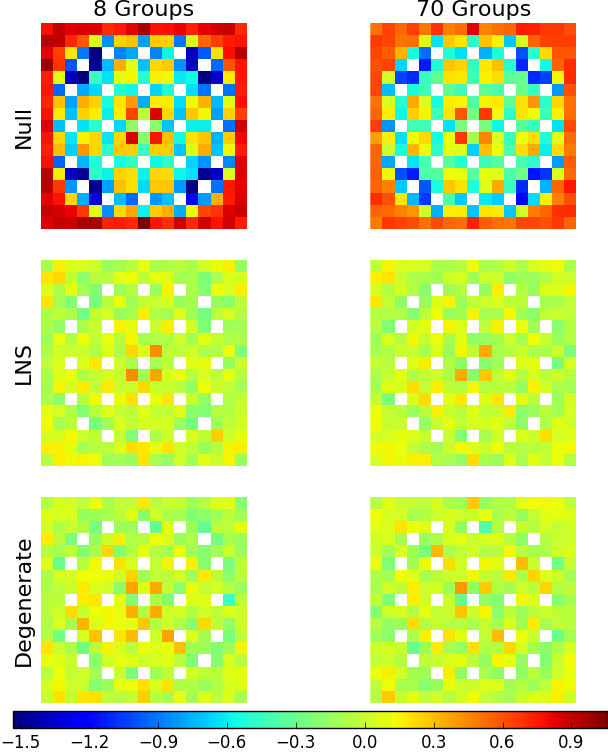
\includegraphics[width=\linewidth]{figures/patterns/lns/assm-16/capt-err}
\vspace{2mm}
\caption[U-238 capture rate errors for a 1.6\% enriched assembly]{U-238 capture rate percent relative errors errors for a 1.6\% enriched assembly with \ac{LNS} spatial homogenization.}
\label{fig:chap9-assm-1.6-lns-capt-err}
\end{figure}

\clearpage

\begin{figure}[h!]
\centering
\includegraphics[width=\linewidth]{figures/patterns/lns/assm-31/capt-err}
\vspace{2mm}
\caption[U-238 capture rate errors for a 3.1\% enriched assembly]{U-238 capture rate percent relative errors errors for a 3.1\% enriched assembly with \ac{LNS} spatial homogenization.}
\label{fig:chap9-assm-3.1-lns-capt-err}
\end{figure}

\clearpage

\begin{figure}[h!]
\centering
\includegraphics[width=\linewidth]{figures/patterns/lns/assm-31-20BPs/capt-err}
\vspace{2mm}
\caption[U-238 capture rate errors for a 3.1\% enriched assembly with 20 BPs]{U-238 capture rate percent relative errors errors for a 3.1\% enriched assembly with 20 \acp{BP} with \ac{LNS} spatial homogenization.}
\label{fig:chap9-assm-3.1-20BPs-lns-capt-err}
\end{figure}

\clearpage

\begin{figure}[h!]
\centering
\includegraphics[width=\linewidth]{figures/patterns/lns/2x2/capt-err}
\vspace{2mm}
\caption[U-238 capture rate errors for a 2$\times$2 colorset]{U-238 capture rate percent relative errors errors for a 2$\times$2 colorset with \ac{LNS} spatial homogenization.}
\label{fig:chap9-2x2-lns-capt-err}
\end{figure}

\clearpage

\begin{figure}[h!]
\centering
\includegraphics[width=\linewidth]{figures/patterns/lns/reflector/capt-err}
\vspace{2mm}
\caption[U-238 capture rate errors for a 2$\times$2 colorset with a reflector]{U-238 capture percent relative errors rate errors for a 2$\times$2 colorset with \ac{LNS} spatial homogenization.}
\label{fig:chap9-reflector-lns-capt-err}
\end{figure}

\clearpage

\begin{figure}[h!]
\centering
\includegraphics[width=\linewidth]{figures/patterns/lns/full-core/capt-err-null}
\vspace{2mm}
\caption[U-238 capture rate errors for \ac{BEAVRS} with null homogenization]{U-238 capture rate absolute errors for the 2D quarter core \ac{BEAVRS} model with null spatial homogenization.}
\label{fig:chap9-full-core-capt-err-null}
\end{figure}

\clearpage

\begin{figure}[h!]
\centering
\includegraphics[width=\linewidth]{figures/patterns/lns/full-core/capt-err-lns}
\vspace{2mm}
\caption[U-238 capture rate absolute errors for \ac{BEAVRS} with LNS homogenization]{U-238 capture rate absolute errors for the 2D quarter core \ac{BEAVRS} model with \ac{LNS} spatial homogenization.}
\label{fig:chap9-full-core-capt-err-lns}
\end{figure}

\clearpage

\begin{figure}[h!]
\centering
\includegraphics[width=\linewidth]{figures/patterns/lns/full-core/capt-err-degenerate}
\vspace{2mm}
\caption[U-238 capture rate absolute errors for \ac{BEAVRS} with degenerate homogenization]{U-238 capture rate absolute errors for the 2D quarter core \ac{BEAVRS} model with degenerate spatial homogenization.}
\label{fig:chap9-full-core-capt-err-degenerate}
\end{figure}

%\begin{figure}[h!]
%\centering
%\begin{subfigure}{.5\textwidth}
%  \centering
%  \includegraphics[width=0.9\linewidth]{figures/patterns/lns/full-core/capt-err-null}
%  \caption{}
%  \label{fig:chap9-full-core-null}
%\end{subfigure}%
%\begin{subfigure}{.5\textwidth}
%  \centering
%  \includegraphics[width=0.9\linewidth]{figures/patterns/lns/full-core/capt-err-null-magnitude}
%  \caption{}
%  \label{fig:chap9-full-core-null-magnitude}
%\end{subfigure}
%\begin{subfigure}{.5\textwidth}
%  \centering
%  \includegraphics[width=0.9\linewidth]{figures/patterns/lns/full-core/capt-err-lns}
%  \caption{}
%  \label{fig:chap9-full-core-lns}
%\end{subfigure}%
%\begin{subfigure}{.5\textwidth}
%  \centering
%  \includegraphics[width=0.9\linewidth]{figures/patterns/lns/full-core/capt-err-lns-magnitude}
%  \caption{}
%  \label{fig:chap9-full-core-lns-magnitude}
%\end{subfigure}
%\begin{subfigure}{.5\textwidth}
%  \centering
%  \includegraphics[width=0.9\linewidth]{figures/patterns/lns/full-core/capt-err-degenerate}
%  \caption{}
%  \label{fig:chap7-pin-1.6}
%\end{subfigure}%
%\begin{subfigure}{.5\textwidth}
%  \centering
%  \includegraphics[width=0.9\linewidth]{figures/patterns/lns/full-core/capt-err-degenerate-magnitude}
%  \caption{}
%  \label{fig:chap7-pin-crgt}
%\end{subfigure}
%\caption[U-238 capture rate errors for the \ac{BEAVRS} quarter core model]{U-238 capture percent relative errors rate errors for the \ac{BEAVRS} quarter core model with \ac{LNS} spatial homogenization.}\label{fig:chap9-full-core-lns-capt-err}
%\end{figure}

%\clearpage


%%%%%%%%%%%%%%%%%%%%%%%%%%%%%%%%%%%%%%%%%%%%%%%%%%%%%%%%%%%%%%%%%%%%%%%%%%%%%%%
\section{MGXS Convergence Rate Analysis}
\label{sec:chap9-convergence}

first paragraph: 
-Fig.~\ref{fig:chap9-converge}
  -batch-wise percentage change for \ac{MGXS} with null, degenerate and \ac{LNS} spatial homogenization
  -explain what ``batch-wise change'' means
-\ac{MGXS} for null changes the least from batch to batch
  -track density in each tally volume (in this case, all pins taken together) is greatest
-\ac{MGXS} for degenerate changes the most from batch to batch
  -track density in each tally volume (in this case, each unique fuel pin instance) is least
-\ac{MGXS} for \ac{LNS} changes less than degenerate but more than null
  -track density is in between since \ac{MGXS} are averaged across groups of like fuel pin instance

second paragraph: key takeaways
-convergence rate (slope) is same for all schemes
-averaging across pins shifts convergence curves to right
-the size/magnitude of the leftward shift depends on the number of pins being averaged across
-hence, the more pins we can average across, the faster we can compute \ac{MGXS} with \ac{MC}

third paragraph: segue into next chapter
-goal should be to best identify groups of pins with like \ac{MGXS}
-\ac{LNS} was used as one scheme
  -demonstrated promise for simple benchmarks
  -illustrated shortcomings for benchmarks with complicated heterogeneties
    -assembly-assembly and assembly-reflector interfaces
  -algorithm could be tweaked to pick up on these effects
    -customizations highly reactor dependent - NOT reactor agnostic
-would be nice to identify adequate pin groupings directly from structural patterns in the \ac{MGXS} data
-will do this in the following chapter

\begin{figure}[h!]
\centering
\begin{subfigure}{.87\textwidth}
  \centering
  \includegraphics[width=\linewidth]{figures/patterns/convergence/assm-16/assm-16-capt}
  \caption{}
  \label{fig:chap9-assm-16-converge}
\end{subfigure}
\begin{subfigure}{.87\textwidth}
  \centering
  \includegraphics[width=\linewidth]{figures/patterns/convergence/full-core/16-enr-capt}
  \caption{}
  \label{fig:chap9-reflector-converge}
\end{subfigure}
\caption[Convergence of pin-wise U-238 capture MGXS]{The batch-wise change of pin-wise U-238 capture \ac{MGXS} (group 27 of 70) for 1.6\% enriched fuel pins in a single assembly (a) and the quarter core \ac{BEAVRS} model (b). The convergence of both the maximum and mean absolute percent change are shown for the degenerate and \ac{LNS} homogenization schemes.}
\label{fig:chap9-converge}
\end{figure}


SUMMARY BOXES!!!
